%%%%%%%%%%%%%%%%%%%%%%%%%%%%%%%%%%%%%%%%%%%%%%%%%%%%%%%%%%%%%%%%%%%%%%%%%%%%%%%%%
% Template: Article
%
% Por: Abrantes Araújo Silva Filho
%      abrantesasf@gmail.com
%
% Citação: Se você gostou deste template, por favor ajude a divulgá-lo mantendo
%          o link para meu repositório GitHub em:
%          https://github.com/abrantesasf/LaTeX
%%%%%%%%%%%%%%%%%%%%%%%%%%%%%%%%%%%%%%%%%%%%%%%%%%%%%%%%%%%%%%%%%%%%%%%%%%%%%%%%%




%%%%%%%%%%%%%%%%%%%%%%%%%%%%%%%%%%%%%%%%%%%%%%%%%%%%%%%%%%%%%%%%%%%%%%%%%%%%%%%%%
%%% Configura o tipo de documento, papel, tamanho da fonte e informações básicas
%%% para as proriedades do PDF/DVIPS e outras propriedades do documento
\RequirePackage{ifpdf}
\ifpdf
  % Classe, língua e tamanho da fonte padrão. Outras opções a considerar:
  %   draft
  %   onecolumn (padrão) ou twocolumn (OU usar o package multicol)
  %   fleqn com ou sem leqno (alinhamento à esquerda das fórmulas e dos números)
  %   oneside (padrão para article ou report) ou twoside (padrão para book)
  \documentclass[pdftex, brazil, 12pt, twoside]{article}
\else
  % Classe, língua e tamanho da fonte padrão. Outras opções a considerar:
  %   draft
  %   onecolumn (padrão) ou twocolumn (OU usar o package multicol)
  %   fleqn com ou sem leqno (alinhamento à esquerda das fórmulas e dos números)
  %   oneside (padrão para article ou report) ou twoside (padrão para book)
  \documentclass[brazil, 12pt]{article}
\fi


%%%%%%%%%%%%%%%%%%%%%%%%%%%%%%%%%%%%%%%%%%%%%%%%%%%%%%%%%%%%%%%%%%%%%%%%%%%%%%%%%
%%% Carrega pacotes iniciais necessários para estrutura de controle e para a
%%% criação e o parse de novos comandos
\usepackage{ifthen}
\usepackage{xparse}


%%%%%%%%%%%%%%%%%%%%%%%%%%%%%%%%%%%%%%%%%%%%%%%%%%%%%%%%%%%%%%%%%%%%%%%%%%%%%%%%%
%%% Configuração do tamanho da página, margens, espaçamento entrelinhas e, se
%%% necessário, ativa a indentação dos primeiros parágrafos.
\ifpdf
  \usepackage[pdftex]{geometry}
\else
  \usepackage[dvips]{geometry}
\fi
\geometry{a4paper, left=2.6cm, right=4.0cm, top=3.0cm, bottom=3.4cm}

\usepackage{setspace}
  %\singlespacing
  \onehalfspacing
  %\doublespacing


%%%%%%%%%%%%%%%%%%%%%%%%%%%%%%%%%%%%%%%%%%%%%%%%%%%%%%%%%%%%%%%%%%%%%%%%%%%%%%%%%
%%% Configurações de cabeçalho e rodapé:
\usepackage{fancyhdr}
\setlength{\headheight}{1cm}
\setlength{\footskip}{1.5cm}
\renewcommand{\headrulewidth}{0.3pt}
\renewcommand{\footrulewidth}{0.0pt}
\pagestyle{fancy}
\renewcommand{\sectionmark}[1]{%
  \markboth{\uppercase{#1}}{}}
\renewcommand{\subsectionmark}[1]{%
  \markright{\uppercase{\thesubsection \hspace{0.1cm} #1}}{}}
\fancyhead{}
\fancyfoot{}
\newcommand{\diminuifonte}{%
    \fontsize{9pt}{9}\selectfont
}
\newcommand{\aumentafonte}{%
    \fontsize{12}{12}\selectfont
}
% Configura cabeçalho e rodapé para documentos TWOSIDE
\fancyhead[EL]{\textbf{\thepage}}
\fancyhead[EC]{}
\fancyhead[ER]{\diminuifonte \textbf{\leftmark}}
\fancyhead[OR]{\textbf{\thepage}}
\fancyhead[OC]{}
\fancyhead[OL]{\diminuifonte \textbf{\rightmark}}
\fancyfoot[EL,EC,ER,OR,OC,OL]{}
% Configura cabeçalho e rodapé para documentos ONESIDE
%\lhead{ \fancyplain{}{sup esquerdo} }
%\chead{ \fancyplain{}{sup centro} }
%\rhead{ \fancyplain{}{\thesection} }
%\lfoot{ \fancyplain{}{inf esquerdo} }
%\cfoot{ \fancyplain{}{inf centro} }
%\rfoot{ \fancyplain{}{\thepage} }


%%%%%%%%%%%%%%%%%%%%%%%%%%%%%%%%%%%%%%%%%%%%%%%%%%%%%%%%%%%%%%%%%%%%%%%%%%%%%%%%%
%%% Configurações de encoding, lingua e fontes:
\usepackage[T1]{fontenc}
\usepackage[utf8]{inputenc}
\usepackage{babel}

% Altera a fonte padrão do documento (nem todas funcionam em modo math):
%   phv = Helvetica
%   ptm = Times
%   ppl = Palatino
%   pbk = bookman
%   pag = AdobeAvantGarde
%   pnc = Adobe NewCenturySchoolBook
\renewcommand{\familydefault}{ppl}


%%%%%%%%%%%%%%%%%%%%%%%%%%%%%%%%%%%%%%%%%%%%%%%%%%%%%%%%%%%%%%%%%%%%%%%%%%%%%%%%%
%%% Carrega pacotes para referências cruzadas, citações dentro do documento,
%%% links para internet e outros.Configura algumas opções.
%%% Não altere a ordem de carregamento dos packages.
\usepackage{varioref}
\ifpdf
  \usepackage[pdftex]{hyperref}
    \hypersetup{
      % Informações variáveis em cada documento (MUDE AQUI!):
      pdftitle={Internet das Coisas},
      pdfauthor={Abrantes Araújo Silva Filho, Brendhom Félix Garcia Brito, Carlos Augusto Caus Couto%
      Eliziel de Paula da Silva, Iuri Alves Contarelli, Victor Luchsinger Lube},
      pdfsubject={Internet das Coisas},
      pdfkeywords={internet das coisas, internet of things, iot, conceitos, histórico, aplicações, riscos, protótipo},
      pdfinfo={
        CreationDate={}, % Ex.: D:AAAAMMDDHH24MISS
        ModDate={}       % Ex.: D:AAAAMMDDHH24MISS
      },
      % Coisas que você não deve alterar se não souber o que está fazendo:
      unicode=true,
      pdflang={pt-BR},
      bookmarksopen=true,
      bookmarksnumbered=true,
      bookmarksopenlevel=5,
      pdfdisplaydoctitle=true,
      pdfpagemode=UseOutlines,
      pdfstartview=FitH,
      pdfcreator={LaTeX with hyperref package},
      pdfproducer={pdfTeX},
      pdfnewwindow=true,
      colorlinks=true,
      citecolor=red,
      linkcolor=red,
      filecolor=cyan,
      urlcolor=blue
    }
\else
  \usepackage{hyperref}
\fi
\usepackage{cleveref}
\usepackage{url}


%%%%%%%%%%%%%%%%%%%%%%%%%%%%%%%%%%%%%%%%%%%%%%%%%%%%%%%%%%%%%%%%%%%%%%%%%%%%%%%%%
%%% Referências bibliográficas
\usepackage[round, semicolon, authoryear]{natbib}
\bibliographystyle{abrantesasf}


%%%%%%%%%%%%%%%%%%%%%%%%%%%%%%%%%%%%%%%%%%%%%%%%%%%%%%%%%%%%%%%%%%%%%%%%%%%%%%%%%
%%% Várias notas de rodapé no mesmo local
%\usepackage[multiple]{footmisc}


%%%%%%%%%%%%%%%%%%%%%%%%%%%%%%%%%%%%%%%%%%%%%%%%%%%%%%%%%%%%%%%%%%%%%%%%%%%%%%%%%
%%% Carrega bibliotecas de símbolos (matemáticos, físicos, etc.), fontes
%%% adicionais, e configura algumas opções
\usepackage{amsmath}
\usepackage{amssymb}
\usepackage{amsfonts}
\usepackage{siunitx}
  \sisetup{group-separator = {.}}
  \sisetup{group-digits = {false}}
  \sisetup{output-decimal-marker = {,}}

% Altera separador decimal via comando, se necessário (prefira o siunitx):
%\mathchardef\period=\mathcode`.
%\DeclareMathSymbol{.}{\mathord}{letters}{"3B}
  

%%%%%%%%%%%%%%%%%%%%%%%%%%%%%%%%%%%%%%%%%%%%%%%%%%%%%%%%%%%%%%%%%%%%%%%%%%%%%%%%%
%%% Carrega packages relacionados à computação
\usepackage{algorithm2e}
\usepackage{algorithmicx}
\usepackage{algpseudocode}
\usepackage{listings}
  \lstset{literate=
    {á}{{\'a}}1 {é}{{\'e}}1 {í}{{\'i}}1 {ó}{{\'o}}1 {ú}{{\'u}}1
    {Á}{{\'A}}1 {É}{{\'E}}1 {Í}{{\'I}}1 {Ó}{{\'O}}1 {Ú}{{\'U}}1
    {à}{{\`a}}1 {è}{{\`e}}1 {ì}{{\`i}}1 {ò}{{\`o}}1 {ù}{{\`u}}1
    {À}{{\`A}}1 {È}{{\'E}}1 {Ì}{{\`I}}1 {Ò}{{\`O}}1 {Ù}{{\`U}}1
    {ä}{{\"a}}1 {ë}{{\"e}}1 {ï}{{\"i}}1 {ö}{{\"o}}1 {ü}{{\"u}}1
    {Ä}{{\"A}}1 {Ë}{{\"E}}1 {Ï}{{\"I}}1 {Ö}{{\"O}}1 {Ü}{{\"U}}1
    {â}{{\^a}}1 {ê}{{\^e}}1 {î}{{\^i}}1 {ô}{{\^o}}1 {û}{{\^u}}1
    {Â}{{\^A}}1 {Ê}{{\^E}}1 {Î}{{\^I}}1 {Ô}{{\^O}}1 {Û}{{\^U}}1
    {œ}{{\oe}}1 {Œ}{{\OE}}1 {æ}{{\ae}}1 {Æ}{{\AE}}1 {ß}{{\ss}}1
    {ű}{{\H{u}}}1 {Ű}{{\H{U}}}1 {ő}{{\H{o}}}1 {Ő}{{\H{O}}}1
    {ç}{{\c c}}1 {Ç}{{\c C}}1 {ø}{{\o}}1 {å}{{\r a}}1 {Å}{{\r A}}1
    {€}{{\euro}}1 {£}{{\pounds}}1 {«}{{\guillemotleft}}1
    {»}{{\guillemotright}}1 {ñ}{{\~n}}1 {Ñ}{{\~N}}1 {¿}{{?`}}1
  }
  

%%%%%%%%%%%%%%%%%%%%%%%%%%%%%%%%%%%%%%%%%%%%%%%%%%%%%%%%%%%%%%%%%%%%%%%%%%%%%%%%%
%%% Ativa suporte extendido a cores
\usepackage[svgnames]{xcolor} % Opções de cores: usenames (16), dvipsnames (64),
                              % svgnames (150) e x11names (300).


%%%%%%%%%%%%%%%%%%%%%%%%%%%%%%%%%%%%%%%%%%%%%%%%%%%%%%%%%%%%%%%%%%%%%%%%%%%%%%%%%
%%% Suporte à importação de gráficos externos
\ifpdf
  \usepackage[pdftex]{graphicx}
\else
  \usepackage[dvips]{graphicx}
\fi


%%%%%%%%%%%%%%%%%%%%%%%%%%%%%%%%%%%%%%%%%%%%%%%%%%%%%%%%%%%%%%%%%%%%%%%%%%%%%%%%%
%%% Suporte à criação de gráficos proceduralmente na LaTeX:
\usepackage{tikz}
  \usetikzlibrary{arrows,automata,backgrounds,matrix,patterns,positioning,shapes,shadows}


%%%%%%%%%%%%%%%%%%%%%%%%%%%%%%%%%%%%%%%%%%%%%%%%%%%%%%%%%%%%%%%%%%%%%%%%%%%%%%%%%
%%% Packages para tabelas
\usepackage{array}
\usepackage{longtable}
\usepackage{tabularx}
\usepackage{tabu}
\usepackage{lscape}
\usepackage{colortbl}  
\usepackage{booktabs}


%%%%%%%%%%%%%%%%%%%%%%%%%%%%%%%%%%%%%%%%%%%%%%%%%%%%%%%%%%%%%%%%%%%%%%%%%%%%%%%%%
%%% Packages ambientes de listas
\usepackage{enumitem}
\usepackage[ampersand]{easylist}


%%%%%%%%%%%%%%%%%%%%%%%%%%%%%%%%%%%%%%%%%%%%%%%%%%%%%%%%%%%%%%%%%%%%%%%%%%%%%%%%%
%%% Packages para suporte a ambientes floats, captions, etc.:
\usepackage{float}
\usepackage{wrapfig}
\usepackage{placeins}
\usepackage{caption}
\usepackage{sidecap}
\usepackage{subcaption}


%%%%%%%%%%%%%%%%%%%%%%%%%%%%%%%%%%%%%%%%%%%%%%%%%%%%%%%%%%%%%%%%%%%%%%%%%%%%%%%%%
%%% Meus comandos específicos:
% Commando para ``italizar´´ palavras em inglês (e outras línguas!):
\newcommand{\ingles}[1]{\textit{#1}}

% Commando para colocar o espaço correto entre um número e sua unidade:
\newcommand{\unidade}[2]{\ensuremath{#1\,\mathrm{#2}}}
\newcommand{\unidado}[2]{{#1}\,{#2}}

% Produz ordinal masculino ou feminino dependendo do segundo argumento:
\newcommand{\ordinal}[2]{%
#1%
\ifthenelse{\equal{a}{#2}}%
{\textordfeminine}%
{\textordmasculine}}


%%%%%%%%%%%%%%%%%%%%%%%%%%%%%%%%%%%%%%%%%%%%%%%%%%%%%%%%%%%%%%%%%%%%%%%%%%%%%%%%%
%%% Hifenização específica quando o LaTeX/Babel não conseguirem hifenizar:
\babelhyphenation{Git-Hub au-to-con-fi-gu-rá-vel i-den-ti-fi-ca-ção quan-do}


%%%%%%%%%%%%%%%%%%%%%%%%%%%%%%%%%%%%%%%%%%%%%%%%%%%%%%%%%%%%%%%%%%%%%%%%%%%%%%%%%
%%%%%%%%%%%%%%%%%%%%%%%%%%%%%%%%%%%%%%%%%%%%%%%%%%%%%%%%%%%%%%%%%%%%%%%%%%%%%%%%%
%%%%%%%%%%%%%%%%%%%%%%%%%%%%%%%%%%%%%%%%%%%%%%%%%%%%%%%%%%%%%%%%%%%%%%%%%%%%%%%%%
%%%%%%%%%%%%%%%%%%%%%%%%%%%%%%%%%%%%%%%%%%%%%%%%%%%%%%%%%%%%%%%%%%%%%%%%%%%%%%%%%
%%%%%%%%%%%%%%%%%%%%%%%%%%%%%% COMEÇA O DOCUMENTO %%%%%%%%%%%%%%%%%%%%%%%%%%%%%%%
%%%%%%%%%%%%%%%%%%%%%%%%%%%%%%%%%%%%%%%%%%%%%%%%%%%%%%%%%%%%%%%%%%%%%%%%%%%%%%%%%
%%%%%%%%%%%%%%%%%%%%%%%%%%%%%%%%%%%%%%%%%%%%%%%%%%%%%%%%%%%%%%%%%%%%%%%%%%%%%%%%%
%%%%%%%%%%%%%%%%%%%%%%%%%%%%%%%%%%%%%%%%%%%%%%%%%%%%%%%%%%%%%%%%%%%%%%%%%%%%%%%%%
%%%%%%%%%%%%%%%%%%%%%%%%%%%%%%%%%%%%%%%%%%%%%%%%%%%%%%%%%%%%%%%%%%%%%%%%%%%%%%%%%
\begin{document}
\title{Internet das Coisas}
\author{Abrantes Araújo Silva Filho \and Brendhom Félix Garcia Brito
  \and Carlos Augusto Caus Couto \and Eliziel de Paula da Silva \and Iuri Alves Contarelli
  \and Victor Luchsinger Lube}
\date{2018-04-19}
\maketitle
% Resolvi não incluir o resumo para o layout do sumário ficar melhor.
\begin{abstract}
  A Internet das Coisas (\ingles{Internet of Things --- IoT}) tem o potencial de
  revolucionar a maneira como nosso cotidiano é percebido e o modo com o qual lidamos
  com objetos comuns que, ao serem conectados à Internet, nos oferecem dados, serviços
  e interatividade sem precedência na história humana. Através da IoT podemos nos
  focar em atividades importantes e contar com dispositivos que realizam tarefas
  rotineiras e enfadonhas (um sistema de irrigação inteligente que ajusta a
  freqüência e o volume de água) ou tarefas especializadas e complexas (dispositivos
  implantáveis que ajudam no controle da glicemia e alertam a equipe médica
  quando uma pessoa está em situação de risco). As aplicações da IoT parecem futuristas
  e distantes, mas muitas já existem e funcionam hoje em dia.
  Este trabalho\footnote{%
  Trabalho Acadêmico do curso de
  \href{https://www.faesa.br/curso/ciencia-da-computacao/}{Ciência da Computação}
  apresentado à \href{https://www.faesa.br/}{FAESA Centro Universitário}, como
  parte das exigências
  da disciplina de Introdução à Computação, sob orientação da prof.ª MSc.\ Renata
  Cristina Laranja Leite.} apresenta
  uma introdução geral sobre o conceito, histórico, aplicações e possíveis riscos
  dessa tecnologia, com o objetivo de fornecer uma visão abrangente dos principais
  componentes do ecossistema da IoT. Também descreve resumidamente um protótipo
  de cofre conectado à Internet que será desenvolvido pelos autores como uma prova
  de conceito da IoT.

  \textbf{Palavras-chave:} Internet das Coisas; Internet of Things;
  IoT; Conceitos; Histórico; Aplicações; Riscos; Protótipo.
\end{abstract}
\tableofcontents


%%%%%%%%%%%%%%%%%%%%%%%%%%%%%%%%%%%%%%%%%%%%%%%%%%%%%%%%%%%%%%%%%%%%%%%%%%%%%%%%%
%%%%%%%%%%%%%%%%%%%%%%%%%%%%%%%%%%%%%%%%%%%%%%%%%%%%%%%%%%%%%%%%%%%%%%%%%%%%%%%%%
%%%%%%%%%%%%%%%%%%%%%%%%%%%%%%%%%%%%%%%%%%%%%%%%%%%%%%%%%%%%%%%%%%%%%%%%%%%%%%%%%
\section{Introdução}
\label{intro}

Nos últimos anos a tecnologia permitiu a criação e o desenvolvimento de dispositivos com a
capacidade de se conectar à Internet e de trocar informações. Esses dispositivos,
segundo \citet[][p.\ 23]{BarbozaTCCIoT2015}, ``são objetos físicos, 'coisas', que passam
a alojar sistemas eletrônicos embarcados com componentes de \ingles{software},
sensores e, principalmente conectividade, que permite a esses objetos trocarem
informações através da rede''.

Apesar de não haver um consenso na definição do campo de ``dispositivos conectados'',
o nome Internet das Coisas --- do inglês \ingles{Internet of Things} (IoT)\footnote{Neste trabalho
  utilizamos a sigla ``IoT'' para indicar todo o ecossistema de dispositivos conectados.} --- passou
a significar todo o ecossistema de \ingles{hardware} e \ingles{software} que
permite a conexão dos dispositivos entre si e à Internet.


%%%%%%%%%%%%%%%%%%%%%%%%%%%%%%%%%%%%%%%%%%%%%%%%%%%%%%%%%%%%%%%%%%%%%%%%%%%%%%%%%
%%%%%%%%%%%%%%%%%%%%%%%%%%%%%%%%%%%%%%%%%%%%%%%%%%%%%%%%%%%%%%%%%%%%%%%%%%%%%%%%%
\subsection{Potencial da IoT}
\label{intro-potencial}

A produção em escala dos dispositivos para IoT com a conseqüente queda no custo
de produção, aliado à enorme distribuição de redes de conectividade \ingles{wireless},
expandiu de forma exponencial as possibilidades de uso e lucratividade com
tal tecnologia.

No ano de 2013 a Cisco estimou que esse potencial
de mercado alcançaria cerca de 14,4 trilhões de dólares em dez anos\footnote{De 2013 a 2022, considerando
o mercado global.}~\citep{CiscoIoTFAQ2013},
e que até 2020 haverá 50,1 bilhões de dispositivos conectados à Internet,
realizando diversas tarefas e serviços~\citep{CiscoIoEConnectionsCounter}.

Além das empresas de tecnologia, grandes consultoras de negócios internacionais
já apontam o enorme potencial da IoT, explicitamente aconselhando
seus clientes a investirem na área.
A Morgan Stanley publicou dois relatórios~\citep{MorganStanleyIoTnow2013,MorganStanleyIoTpersonal2014}
que apontam enorme potencial de ganhos, e a \citet[][p.\ 4]{OliverWymanIoT2015} classifica
a IoT como ``uma nova revolução capaz de romper os modelos de negócios tradicionais''.

Até mesmo governos, que geralmente são mais lentos na adoção de novas tecnologias, já
se movimentam para estudar, testar e implantar soluções concetadas. O Reino Unido,
por exemplo, estabeleceu para si a meta de se tornar, através do investimento em IoT,
a ``nação mais digital entre os componentes do G8\footnote{França, Alemanha, Reino Unido,
  Japão, Canadá, Itália, Estados Unidos e Rússia (esta foi afastada recentemente sob
  a acusação de violaão da soberania nacional da Ucrânia).}'' e 
``o líder mundial no desenvolvimento e implementação da IoT''~\citep[][p.\ 5]{UKGOSWalportIoT2014}.

E por que toda essa agitação em torno da IoT? Porque as suas aplicações
são praticamente inesgotáveis, variando desde uma simples
\ingles{Smart-TV} capaz de se conectar à Internet e atualizar a programação de
filmes disponíveis, de um simples sistema de irrigação de jardim capaz de
obter a previsão de chuva a partir de serviços na Internet e ajustar a periodicidade
na qual a grama será molhada, até dispositivos complexos como um marca-passo cardíaco
capaz de informar automaticamente ao médico ou uma equipe de emergência uma possível
disfunção miocárdica que exija tratamento imediato.


%%%%%%%%%%%%%%%%%%%%%%%%%%%%%%%%%%%%%%%%%%%%%%%%%%%%%%%%%%%%%%%%%%%%%%%%%%%%%%%%%
%%%%%%%%%%%%%%%%%%%%%%%%%%%%%%%%%%%%%%%%%%%%%%%%%%%%%%%%%%%%%%%%%%%%%%%%%%%%%%%%%
\subsection{Objetivos deste trabalho}
\label{intro-objetivos}

Este trabalho pretende apresentar uma visão geral do campo da IoT, incluindo os
seguintes conteúdos:

\begin{itemize}[noitemsep]
\item Conceitos e principais definições a respeito da IoT;
\item Ecossistema de \ingles{hardware} e \ingles{software};
\item Histórico;
\item Aplicações;
\item Riscos e perigos;
\item Tecnologias utilizadas.
\end{itemize}

Também será apresentada uma breve descrição de um protótipo de
cofre conectado à Internet, utilizando-se um Arduino\footnote{\url{https://www.arduino.cc/}},
que será desenvolvido pelos autores como uma prova de conceito da IoT.


%%%%%%%%%%%%%%%%%%%%%%%%%%%%%%%%%%%%%%%%%%%%%%%%%%%%%%%%%%%%%%%%%%%%%%%%%%%%%%%%%
%%%%%%%%%%%%%%%%%%%%%%%%%%%%%%%%%%%%%%%%%%%%%%%%%%%%%%%%%%%%%%%%%%%%%%%%%%%%%%%%%
%%%%%%%%%%%%%%%%%%%%%%%%%%%%%%%%%%%%%%%%%%%%%%%%%%%%%%%%%%%%%%%%%%%%%%%%%%%%%%%%%
\section{O que é IoT?}
\label{o-que-e-iot}


%%%%%%%%%%%%%%%%%%%%%%%%%%%%%%%%%%%%%%%%%%%%%%%%%%%%%%%%%%%%%%%%%%%%%%%%%%%%%%%%%
%%%%%%%%%%%%%%%%%%%%%%%%%%%%%%%%%%%%%%%%%%%%%%%%%%%%%%%%%%%%%%%%%%%%%%%%%%%%%%%%%
\subsection{Definição e conceitos}
\label{o-que-e-iot-definicao}

Não existe um consenso estabelecido sobre o que realmente é a IoT e qual a melhor
maneira de definí-la. Isso ocorre devido a relativa pouca idade e maturação do
campo, devido às diferentes visões dos dispositivos pioneiros de IoT, e devido
ao praticamente ilimitado potencial de uso para diferentes atividades e serviços
em diversas áreas (indústria, doméstica, saúde, financeira, engenharia,
energia, transporte e muitas
outras). Se a IoT estará presente em tudo e servirá para tudo, como
definí-la precisamente?

Inicialmente vamos eliminar uma visão simplória e quase caricata da IoT: a
``geladeira conectada que compra leite fresco'' (ver Figura~\ref{fig:smart-geladeira}).
\citet[][p.\ 6]{UKGOSWalportIoT2014}
argumenta que esse tipo de estereótipo somente contribui para ``trivializar
a importância da IoT'' e mascarar o verdadeiro potencial de impacto na sociedade.
Eletrodomésticos conectados são uma pequena parte da IoT, mas não a mais
importante.

\begin{figure}[h]
  \begin{center}
    \caption{``A porta-voz da Samsung, Kai Madden, exibe o recurso de conectividade em
      uma geladeira inteligente da fabricante Samsung''~\citep{BajarinIoE2014}}
    \label{fig:smart-geladeira}
    \fbox{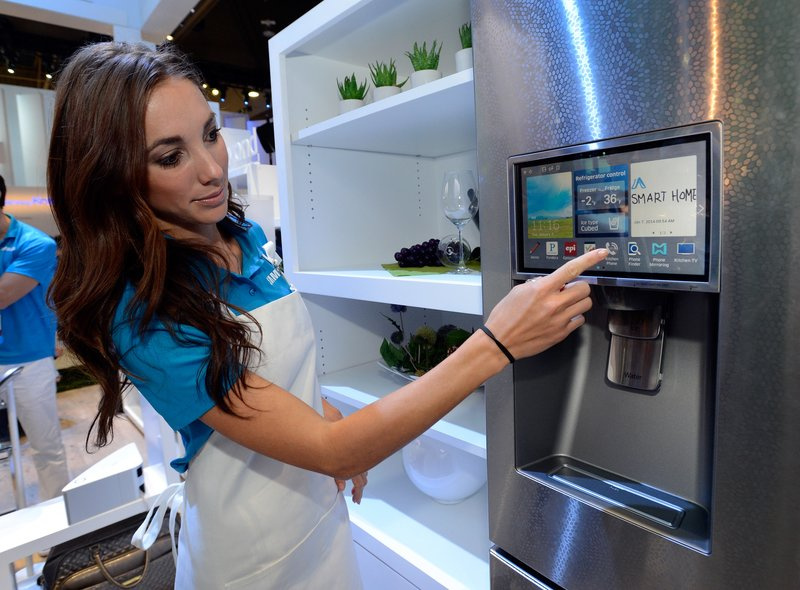
\includegraphics[scale=0.9]{imagens/geladeira.jpeg}}

    \footnotesize{Fonte:~\citet{BajarinIoE2014}}%,
%      disponível em \url{http://time.com/539/the-next-big-thing-for-tech-the-internet-of-everything/}}
  \end{center}
\end{figure}

Se a IoT não se resume a eletrodomésticos conectados, o que ela é de fato? As
grandes empresas de tecnologia definem IoT do seguinte modo:

\begin{itemize}
\item \emph{\textbf{Systeme, Anwendungen und Produkte in der Datenverarbeitung (SAP)}}:
  ``A Internet das Coisas é uma rede de objetos físicos --- veículos,
  máquinas, eletrodomésticos e outros --- que usam sensores e APIs\footnote{%
    Interface de Programação de Aplicações, do inglês \ingles{Application Programming
    Inferface} (API).}
  para conectar e trocar dados na Internet''~\citep{SAPWhatIoT};
\item \emph{\textbf{Statistical Analysis System (SAS)}}: ``A Internet das Coisas é o
  conceito de objetos do cotidiano --- de
  máquinas industriais à dispositivos vestíveis\footnote{%
    Neologismo derivado da palavra inglesa \ingles{wearable}, usado para identificar
    alguma tecnologia que pode ser vestida como uma roupa ou acessório.}
  --- usando sensores embutidos para coletar
  dados e tomar uma ação sobre esses dados através da rede''\citep{SASWhatIoT};
\item \emph{\textbf{International Business Machines (IBM)}}: ``A Internet das Coisas
  refere-se à variedade crescente
  de dispositivos conectados que enviam dados através da Internet. Uma 'coisa' é qualquer
  objeto com eletrônica embarcada que pode transferir dados em uma rede --- sem nenhuma
  interação humana''~\citep{IBMWhatIsIoT,IBMWhatsonIoT};
\item \emph{\textbf{Cisco}}: ``A Internet das Coisas (IoT) refere-se simplesmente à conexão
  em rede de objetos físicos''~\citep{CiscoIoTVS2013};
\item \emph{\textbf{Amazon}}: ``Um sistema de dispositivos ubíquos conectando o mundo
  físico à nuvem''~\citep{AmazonIoT};
\item \emph{\textbf{Microsoft}}: embora a \ingles{Microsoft} não defina explicitamente o que
  ela entende por IoT, em um vídeo institucional sobre a plataforma \emph{Microsoft IoT}
  podemos deduzir que o conceito de IoT envolve conectar as partes mais vitais de
  seu negócio (pessoas, ativos, processos e sistemas), do chão de fábrica aos ``campos''
  para aumentar o alcançe da empresa e fazer melhor uso dos recursos~\citep{MicrosoftIoT};
\item \emph{\textbf{Google}}: a empresa também não fornece uma definição explícita mas
  sua plataforma \emph{Google Cloud IoT Core} está voltada à ``conexão segura, coleta e
  gerenciamento de dados a partir de milhões de dispositivos globalmente dispersos [\ldots]
  para processar, analisar e visualizar dados em tempo real para suportar o aumento
  da eficiência operacional''~\citep{GoogleWhatsIoT}.
\end{itemize}

Um grande esforço de entendimento e conceituação da IoT foi realizado pelo \ingles{Institute
  of Electrical and Electronics Engineers (IEEE)}, que reconheceu a grande importância
do tema~\citep{IEEEIoTReport}, revisou a definição de IoT
de várias organizações, projetos de pesquisa, governos e instituições de ensino, e publicou
em 2015 sua própria definição de IoT no
relatório\footnote{\url{https://iot.ieee.org/definition.html}}\textsuperscript{, }\footnote{O IEEE revisou
  as definições e conceituações de IoT de 8 organismos internacionais de padronização, 8 projetos
  de pesquisa em IoT, 3 iniciativas de governos, 7 relatórios institucionais de empresas e
  consultorias, 5 livros que tratam exclusivamente de IoT e 3 definições fornecidas por indústrias
que lidam com IoT.}
``\ingles{Towards a definition of
  the Internet of Things (IoT)}''~\citep{IEEEIoTDefinition}. A definição proposta
pelo IEEE é a seguinte:

\begin{quote}
  ``A Internet das Coisas (IoT) é uma rede complexa, auto-configurá-vel e adaptativa,
  que interconecta 'coisas' à Internet através do uso de protocolos de comunicação
  padronizados. As coisas interconectadas têm representação física ou virtual no mundo
  digital, com capacidades sensoriais, de atuação e programabilidade, e são unicamente
  identificáveis. A representação contém informação sobre a coisa incluindo sua identidade,
  status, localização ou qualquer outra informação relevante, privada, social ou
  empresarial. A coisa oferece serviços, com ou sem a intervenção humana, através
  da exploração de sua identificação única, dados capturados, comunicação e capacidade
  de atuação. Os serviços são explorados através do uso de interfaces inteligentes e
  estão disponíveis em qualquer lugar, a qualquer hora e para qualquer um ou qualquer
  coisa, levando em consideração questões de segurança.''~\citep[][p.\ 74]{IEEEIoTDefinition}
\end{quote}

Dissecando a definição da IEEE podemos compreender melhor cada parte da IoT:

\begin{enumerate}
\item \emph{\textbf{Coisa}}: é qualquer dispositivo que possa ser conectado
  à Internet, variando desde um minúsculo sensor até um carro ou outro
  grande equipamento, e que tenha capacidade sensorial, de atuação ou de
  programabilidade;
\item \emph{\textbf{Identificação única}}: cada coisa deve ser unicamente
  identificável na Internet pois só assim pode-se captar dados relevantes
  e oferecer serviços importantes para cada um, individualmente;
\item \emph{\textbf{Ubiquidade}}: as coisas e os serviços por elas disponibilizados
  devem estar disponíveis em qualquer lugar, a qualquer hora e para qualquer um
  ou qualquer coisa (note-se que uma coisa pode oferecer serviços para outras
  coisas);
\item \emph{\textbf{Rede}}: as coisas conversam, trocam dados e oferecem
  serviços através de uma rede complexa, atualmente a Internet;
\item \emph{\textbf{Autonomia}}: as coisas devem ser capazes de
  obter dados e oferecer serviços sem a intervenção humana (não excluindo
  a possibilidade da participação humana ativa também);
\item \emph{\textbf{Segurança}}: toda essa atividade de coleta e troca de
  dados via rede resulta em desafios imensos relacionados à segurança e
  privacidade das informações, e as questões de segurança devem ser
  priorizadas.
\end{enumerate}


%%%%%%%%%%%%%%%%%%%%%%%%%%%%%%%%%%%%%%%%%%%%%%%%%%%%%%%%%%%%%%%%%%%%%%%%%%%%%%%%%
%%%%%%%%%%%%%%%%%%%%%%%%%%%%%%%%%%%%%%%%%%%%%%%%%%%%%%%%%%%%%%%%%%%%%%%%%%%%%%%%%
\subsection{Ecossistema da IoT}
\label{o-que-e-iot-ecossistema}

Todas as coisas conectadas à internet, incluindo todo o \ingles{hardware}
e \ingles{software} formam o ``ecossistema da IoT''. Esse ecossistema é ilustrado em maiores
detalhes na Figura~\ref{fig:ecossistema1} (página~\pageref{fig:ecossistema1}),
e, em uma visão mais abrangente e de alto nível, na Figura~\ref{fig:ecossistema2}
(página~\pageref{fig:ecossistema2}).

\begin{figure}[h]
  \begin{center}
    \caption{Ecossistema, características e escopo da IoT}
    \label{fig:ecossistema1}
    \fbox{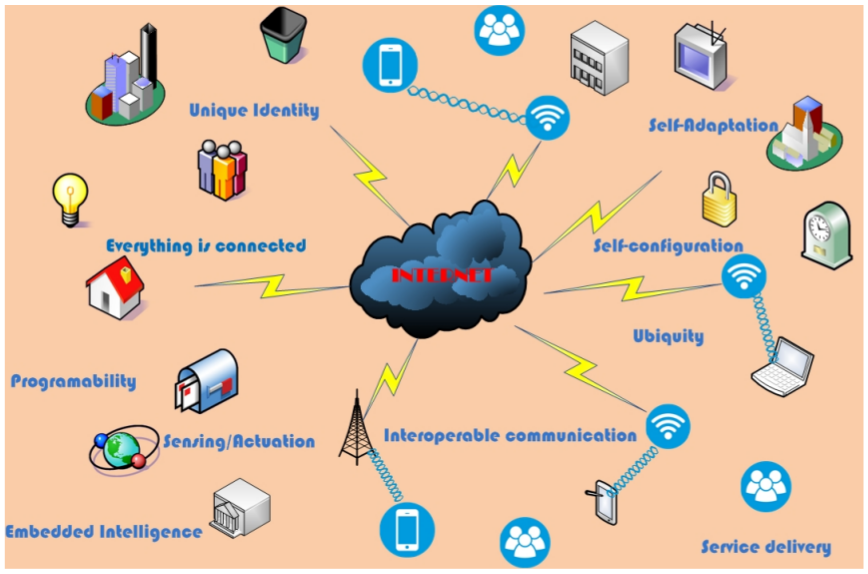
\includegraphics[scale=0.4]{imagens/ecossistema1.png}}
    
    \footnotesize{Fonte:~\citet[][p.\ 74]{IEEEIoTDefinition}}
  \end{center}
\end{figure}

\begin{figure}[h]
  \begin{center}
    \caption{Visão de alto nível do ecossistema da IoT}
    \label{fig:ecossistema2}
    \fbox{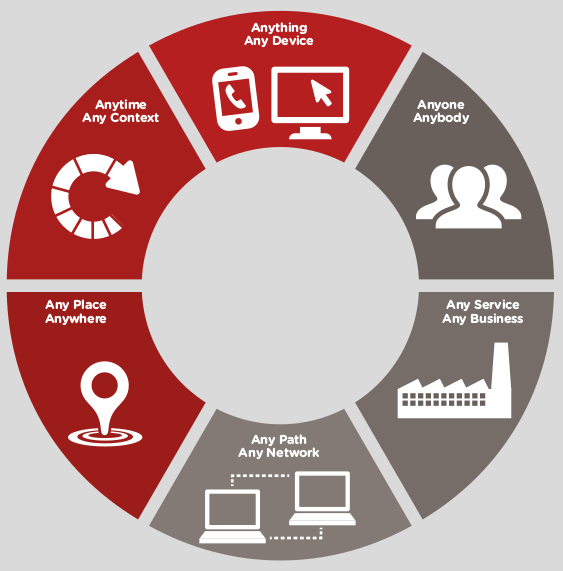
\includegraphics[scale=0.5]{imagens/ecossistema2.png}}
    
    \footnotesize{Fonte:~\citet[][p.\ 13]{UKGOSWalportIoT2014}}
  \end{center}
\end{figure}

O \ingles{hardware} inclui os próprios dispositivos, sensores, atuadores,
servidores de processamento, servidores de armazenamento de dados,
infraestrutura de rede, infraestrutura de nuvem, equipamentos de \ingles{backup}, etc.
Enfim, inclui tudo o que é necessário para manter a estrutura da IoT funcionando.

O \ingles{software} inlcui os sistemas embarcados nos dispositivos, os sistemas
nos servidores, os sistemas de coleta e análise de dados ou qualquer outro
sistema ou programa para que a IoT funcione adequadamente.

Alguns autores~\citep{UKGOSWalportIoT2014,IEEEIoTDefinition,BarbozaTCCIoT2015}
identificam, a grosso modo, dois ``tamanhos'', ou ``escalas'' de ecossistemas
para as aplicações da IoT: pequena ou grande escala.
O que diferencia entre essas duas é a comlexidade em termos de:

\begin{itemize}[noitemsep]
\item Número e diversidade de dispositivos conectados;
\item Propriedade e gerenciamento das coisas e dispositivos.
\end{itemize}

Um ecossistema IoT de \emph{pequena escala} corresponde à uma rede de dispositivos
pouco complexa, com relativamente poucos dispositivos e, principalmente, com
um único proprietário gerenciador. Aqui se encaixam as soluções
de IoT de um único fabricante. Por exemplo: sistemas para a irrigação de jardins
que utilizam dados de previsão do tempo, sistemas em veículos que indicam ao
motorista a necessidade de manutenção preventiva, sistemas em marca-passos cardíacos
que avisam à equipe médica se algum problema ocorrer.

Por outro lado, um ecossistema IoT de \emph{grande escala} corresponde à uma rede
de dispositivos muito complexa, com muitos e diversos dispositivos e, principalmente, com
diversos proprietários e gerenciadores (que podem até não ter relacionamentos
explícitos entre eles). Segundo o \citet[][p.\ 75]{IEEEIoTDefinition}, ``nesse contexto,
a complexidade torna-se dominante e elementos como escalabilidade, lógica distribuída,
etc., tornam-se essenciais. Todas as abordagens tradicionais para gerenciamento
de confiança, nomeação, descoberta, etc., devem ser completamente repensadas''.

As soluções de pequena escala, apesar do nome, já causam profundo impacto na sociedade
mas o maior potencial para a IoT será quando for possível conectar todos os dispositivos,
de todos os fabricantes, em um ecossistema golbal de grande escala~\citep{UKGOSWalportIoT2014,IEEEIoTDefinition,BhattIoT,IEEEIoTReport,McKinseyIoTHype,MoolayilIoT2016,RajIoT2017,OliverWymanIoT2015,SAPFutureIoT,CiscoIoEPublicSectorOpportunity,CiscoIoTFAQ2013,CiscoIoTVS2013,CiscoIoEPublicSectorEconomicAnalysis,CiscoIoESurvey2013,CiscoIoEValuePrivate2013,CiscoIoEValuePublic2013}.

Obviamente, apesar do grande potencial em conectar todos os dispositivos, de todos
os fabricantes, em uma grande rede comum de troca de informações e prestação de
serviços, existem grandes obstáculos a serem superados até que essa visão de futuro
possa ser alcançada \citep{UKGOSWalportIoT2014}, como a falta de padronização dos
protocolos de comunicação entre dispositivos de diversos fabricantes.


%%%%%%%%%%%%%%%%%%%%%%%%%%%%%%%%%%%%%%%%%%%%%%%%%%%%%%%%%%%%%%%%%%%%%%%%%%%%%%%%%
%%%%%%%%%%%%%%%%%%%%%%%%%%%%%%%%%%%%%%%%%%%%%%%%%%%%%%%%%%%%%%%%%%%%%%%%%%%%%%%%%
\subsection{Breve histórico}
\label{o-que-e-iot-historia}

Pode-se afirmar que a história da IoT está intimamente ligada ao desenvolvimento
da tecnologia de \ingles{Radio-Frequency Identification (RFID)}, cujas raízes
tecnológicas podem ser verificáveis desde a segunda guerra mundial~\citep{IEEEIoTDefinition}.
Os países em guerra já utilizavam radares para detectar a aproximação de aviões,
mas não existia um jeito de dizer se os aviões eram de inimigos se aproximando
ou se eram aviões amigos retornando de uma missão. Os alemães foram os
primeiros a descobrir que, ``se os pilotos executassem manobras de 'rolamento'
com os aviões, isso alterava o sinal do radar e permita aos operadores em terra
saber se os aviões eram alemães ou se eram aviões inimigos''~\citep[][p.\ 8]{IEEEIoTDefinition}.
Essencialmente isso era o primeiro sistema de RFID passivo.

Os britânicos logo desenvolveram um sistema ativo de identificação: ``quando
um avião britânico recebia um sinal de radares britânicos, ele repondia através
do \emph{broadcast} de um sinal que era percebido pelos operadores em terra
como um avião amigo''~\citep[][p.\ 8]{IEEEIoTDefinition}.

Segundo o~\citet[][p.\ 8]{IEEEIoTDefinition} a tecnologia RFID funciona basicamente
através do mesmo conceito: ``um sinal é enviado a um tipo de \emph{transponder}
que 'acorda' e ou reflete de volta (RFID passivo) ou realiza
um \emph{broadcast} (RFID ativo) de um sinal''.

Após a guerra, durante as décadas de 1950 e 1960, cientistas e acadêmicos
continuaram a desenvolver tecnologias de rádio-freqüência para identificar
objetos remotamente. Empresas começaram a comercializar sistemas anti-furto
que funcionavam com uma \ingles{tag} eletrônica capaz de informar se o produto
foi pago ou não. Esse sitema, em uso ainda hoje, é composto por \ingles{tags}
que armazenam apenas 1 \ingles{bit} --- 0 (o produto foi pago) ou 1 (o produto não
foi pago) --- e leitores de rádio-freqüência que são instalados nas portas
das lojas~\citep{IEEEIoTDefinition}.

Outros avanços importantes da área de identificação por rádio-freqüência, que
contribuíram para o desenvolvimento da IoT, foram:

\begin{itemize}
\item \emph{\textbf{RFID ativo com memória regravável}}: a primeira patente de um sistema de RFID ativo,
  com memória regravável foi obtida por Mario W. Cardullo, em 1973. Maiores informações
  sobre essa tecnologia podem ser encontradas no artigo de \citet{CardulloRFIDGenesis2003};
\item \emph{\textbf{Cartões fechadura}}: também em 1973, Charles Walton desenvolveu um sistema
  de cartões plásticos com \ingles{transponders} RFID embutidos, capazes de abrir
  portas sem a necessidade de chaves~\citep{IEEEIoTDefinition}. Esse sistema é
  utilizado ainda hoje em hotéis, por exemplo;
\item \emph{\textbf{Sistemas automáticos de pagamento de pedágio}}: durante a década de 1970,
  cientistas do \emph{Los Alamos National Laboratory} desenvolveram uma tecnologia
  para rastrear o transporte de material de bombas nucleares, usando RFIDs com
  capacidade de armazenar maiores informações. Em 1980 esses mesmos cientistas
  fundaram uma empresa e passaram a vender essa tecnologia, agora voltada
  para uso civil, em um sistema de pagamento automático de pedagios~\citep{IEEEIoTDefinition};
\item \emph{\textbf{Rastreamento de gado}}: os cientistas do \emph{Los Alamos National Laboratory}
  também desenvolveram um sistema de ``rastreamento e identificação única voltado
  para gado, para monitorar a localização dos animais e as doses de hormônios e
  vacinas que eles já tinham recebido''~\citep[][p.\ 8--9]{IEEEIoTDefinition}.
\end{itemize}

A aplicação da tecnologia RFID foi sendo
expandida e não servia mais só para identificar um objeto, mas, também, armazenar
dados sobre esse mesmo objeto. Isso era um grande avanço, mas gerava um problema:
armazenar diversos dados em uma \ingles{tag} RFID levava ao aumento do custo
unitário. A idéia era boa, mas era necessário alguma inovação que barateasse o
sistema.

Essa inovação começou a surgir em 1990: no início da década de 1990
a IBM patenteou um sistema de \emph{Ultra-High Frequency} (UHF) RFID, tornando
possível que a leitura dos dados da \emph{tag} fosse feita a uma distância maior
do que até então era possível e com uma rápida velocidade de
transferência~\citep{IEEEIoTDefinition}.

Em 1999 foi fundado, no \ingles{Massachusetts Institute of Technology} (MIT), um
laboratório de inovação chamado de \emph{Auto-ID Center}, cujo objetivo era
desenvolver inovação na área de identificação por rádio-freqüência baseando-se
na tecnologia de UHF RFID desenvolvida pela IBM~\citep{IEEEIoTDefinition}.

Dois cientistas do \ingles{Auto-ID Center},
\emph{\textbf{David Brock}} e \emph{\textbf{Sanjay Sarma}}, foram os pioneiros em investigar a possibilidade
de usar \ingles{tags} UHF RFID de baixo custo em todos os produtos da cadeia
de suprimento. ``A idéia deles era colocar apenas o número de série de cada produto
na \ingles{tag}, barateando seu custo, e manter os dados detalhados de cada
produto em um banco de dados que seria acessível pela Internet''~\citep[][p.\ 9]{IEEEIoTDefinition}.

Ao retirarem os dados detalhados das \ingles{tags} e colocá-los em um banco
de dados acessível pela Internet, estavam lançadas as bases para o desenvolvimento de
dispositivos que se conectavam à rede para ler e/ou fornecer informações.
Assim nasceu a conexão das coisas com a Internet.

Para Roberti, citado em \citet[][p.\ 9]{IEEEIoTDefinition}:
\begin{quote}
``Sarma e Brock
essencialmente mudaram a maneira como as pessoas pensavam sobre o RFID na
cadeia de suprimentos. Antes, as \ingles{tags} eram um banco de dados móvel
que carregavam informações sobre o produto à medida em que esse produto
seguia seu curso. \textbf{Sarma e Brock tornaram o RFID em uma tecnologia de rede
  através da ligação de objetos com a Internet através das \ingles{tags}}.''
\end{quote}

A criação do termo \ingles{Internet of Things (IoT)} é atualmente creditada à Kevin Ashton,
na época o diretor executivo do \ingles{Auto-ID Center}, mas existe uma certa
controvérsia quanto a isso pois segundo Daniel Engels (também um dos
diretores desse centro), citado por~\citet[][p.\ 10]{IEEEIoTDefinition},
o termo foi usado pela primeira vez em 1997 em uma publicação da
\ingles{International Telecommunication Union (ITU)}, enquanto Kevin Ashton afirmou
que cunhou o termo somente em 1999~\citep{AshtonIoT2009,PressIoT2014}.


%%%%%%%%%%%%%%%%%%%%%%%%%%%%%%%%%%%%%%%%%%%%%%%%%%%%%%%%%%%%%%%%%%%%%%%%%%%%%%%%%
%%%%%%%%%%%%%%%%%%%%%%%%%%%%%%%%%%%%%%%%%%%%%%%%%%%%%%%%%%%%%%%%%%%%%%%%%%%%%%%%%
\subsection{Outros conceitos relacionados à internet das coisas}
\label{o-que-e-iot-outros-tipos}

É importante salientar que exitem outros termos e tecnologias relacionadas à
IoT que tratam de coisas semelhantes. Esses outros termos às vezes são usados
como sinônimos de IoT, outras vezes como complementares ou referentes a uma
parte específica do ecossistema da IoT, causando uma certa confusão. Esta
seção explicará brevemente os principais termos alternativos, sem entrar em
maiores detalhes de cada um pois isso foge ao escopo deste trabalho.


%%%%%%%%%%%%%%%%%%%%%%%%%%%%%%%%%%%%%%%%%%%%%%%%%%%%%%%%%%%%%%%%%%%%%%%%%%%%%%%%%
\subsubsection{\ingles{Internet of Everything} (IoE)}
\label{o-que-e-iot-outros-tipos-ioe}

Alguns autores e empresas fazem uma diferenciação entre a \ingles{Internet of Things} (IoT)
e a \ingles{Internet
  of Everything} (IoE), sendo esta ``a conexão em rede de pessoas, processos,
dados e coisas'', e aquela simplesmente ``a conexão em rede de coisas
e dados''~\citep{CiscoIoEPublicSectorOpportunity,CiscoIoTVS2013,CiscoIoTFAQ2013}.
Assim, a IoE seria uma ``evolução'' da IoT, cujo escopo e potencial
são maiores. Segundo \citet{HebraIoTIoE2015} o futuro da IoT caminha para
ser a IoE, trazendo enormes vantagens e benefícios.

A IoE seria uma maneira de incluir tudo o que pode ser conectado, não apenas
coisas e dados, mas algo bem maior e global~\citep{LuethIoT2014,BajarinIoE2014}.


%%%%%%%%%%%%%%%%%%%%%%%%%%%%%%%%%%%%%%%%%%%%%%%%%%%%%%%%%%%%%%%%%%%%%%%%%%%%%%%%%
\subsubsection{\ingles{Machine-to-Machine Communication} (M2M)}
\label{o-que-e-iot-outros-tipos-m2m}

Quando duas ou mais máquinas ou entidades do mesmo tipo têm a capacidade de se
comunicarem de forma autônoma, sem a presença ou intervenção humana, ocorre o que
é chamado de comunicação direta máquina-a-máquina (comunicação M2M). O
principal objetivo da comunicação M2M é poder ``automatizar decisões e
processos''~\citep[][p.\ 12]{IEEEIoTDefinition}.

Apesar de pouco conhecida de modo geral, a comunicação M2M já está em uso há
vários anos no setor de telecomunicações e, hoje, com a explosão da conectividade
móvel e a IoT, muito mais dados e máquinas estão fazendo parte desse sistema
de troca de informações~\citep{LuethIoT2014}.


%%%%%%%%%%%%%%%%%%%%%%%%%%%%%%%%%%%%%%%%%%%%%%%%%%%%%%%%%%%%%%%%%%%%%%%%%%%%%%%%%
\subsubsection{\ingles{Industrial Internet of Things} (IIoT)}
\label{o-que-e-iot-outros-tipos-iiot}

É um termo mais abrangente que a M2M pois envolve, não apenas a comunicação
máquina-a-máquina, mas também a comunicação com interfaces humanas~\citep{LuethIoT2014}
integrando máquinas complexas com \ingles{software} e sensores em rede.


%%%%%%%%%%%%%%%%%%%%%%%%%%%%%%%%%%%%%%%%%%%%%%%%%%%%%%%%%%%%%%%%%%%%%%%%%%%%%%%%%
\subsubsection{\ingles{Web of Things} (WoT)}
\label{o-que-e-iot-outros-tipos-wot}

\ingles{Web of Things} ``é um conjunto de
arquitetura de \ingles{software} e padrões de programação que permitem que
objetos do mundo real façam parte da \ingles{world wide web}''~\citep{LuethIoT2014}.
É assim um conceito mais restrito do que a IoT pois está focada
somente em \ingles{software}.


%%%%%%%%%%%%%%%%%%%%%%%%%%%%%%%%%%%%%%%%%%%%%%%%%%%%%%%%%%%%%%%%%%%%%%%%%%%%%%%%%
\subsubsection{\ingles{Industry 4.0}}
\label{o-que-e-iot-outros-tipos-industry-4.0}

O temo \ingles{Industry 4.0} (ou manufatura ou indústria 4.0) está sendo
utilizado para descrever ``conceitos de conectividade em um contexto industrial,
indo além e incluindo mudanças reais
no mundo físico tais como o uso de tecnologias de impressão 3D ou o uso de realidade
virtual ou aumentada no processo de industrialização''~\citep{LuethIoT2014}.


%%%%%%%%%%%%%%%%%%%%%%%%%%%%%%%%%%%%%%%%%%%%%%%%%%%%%%%%%%%%%%%%%%%%%%%%%%%%%%%%%
\subsubsection{O conjunto dos outros ``tipos'' de internet das coisas}
\label{o-que-e-iot-outros-tipos-conjunto}

Uma figura esquemática simples e objetiva do que é cada ``tipo'' de internet das coisas
discutida nesta seção é fornecida por ~\citet{LuethIoT2014}. Nesse esquema
(ver Figura~\ref{fig:outras-iot}) pode-se
perceber de maneira objetiva o escopo de cada tecnologia e como cada uma se relaciona
com as outras.

\begin{figure}[H]
  \begin{center}
    \caption{Relações entre IoT, IoE, M2M, IIoT, WoT e Indústria 4.0}
    \label{fig:outras-iot}
    \fbox{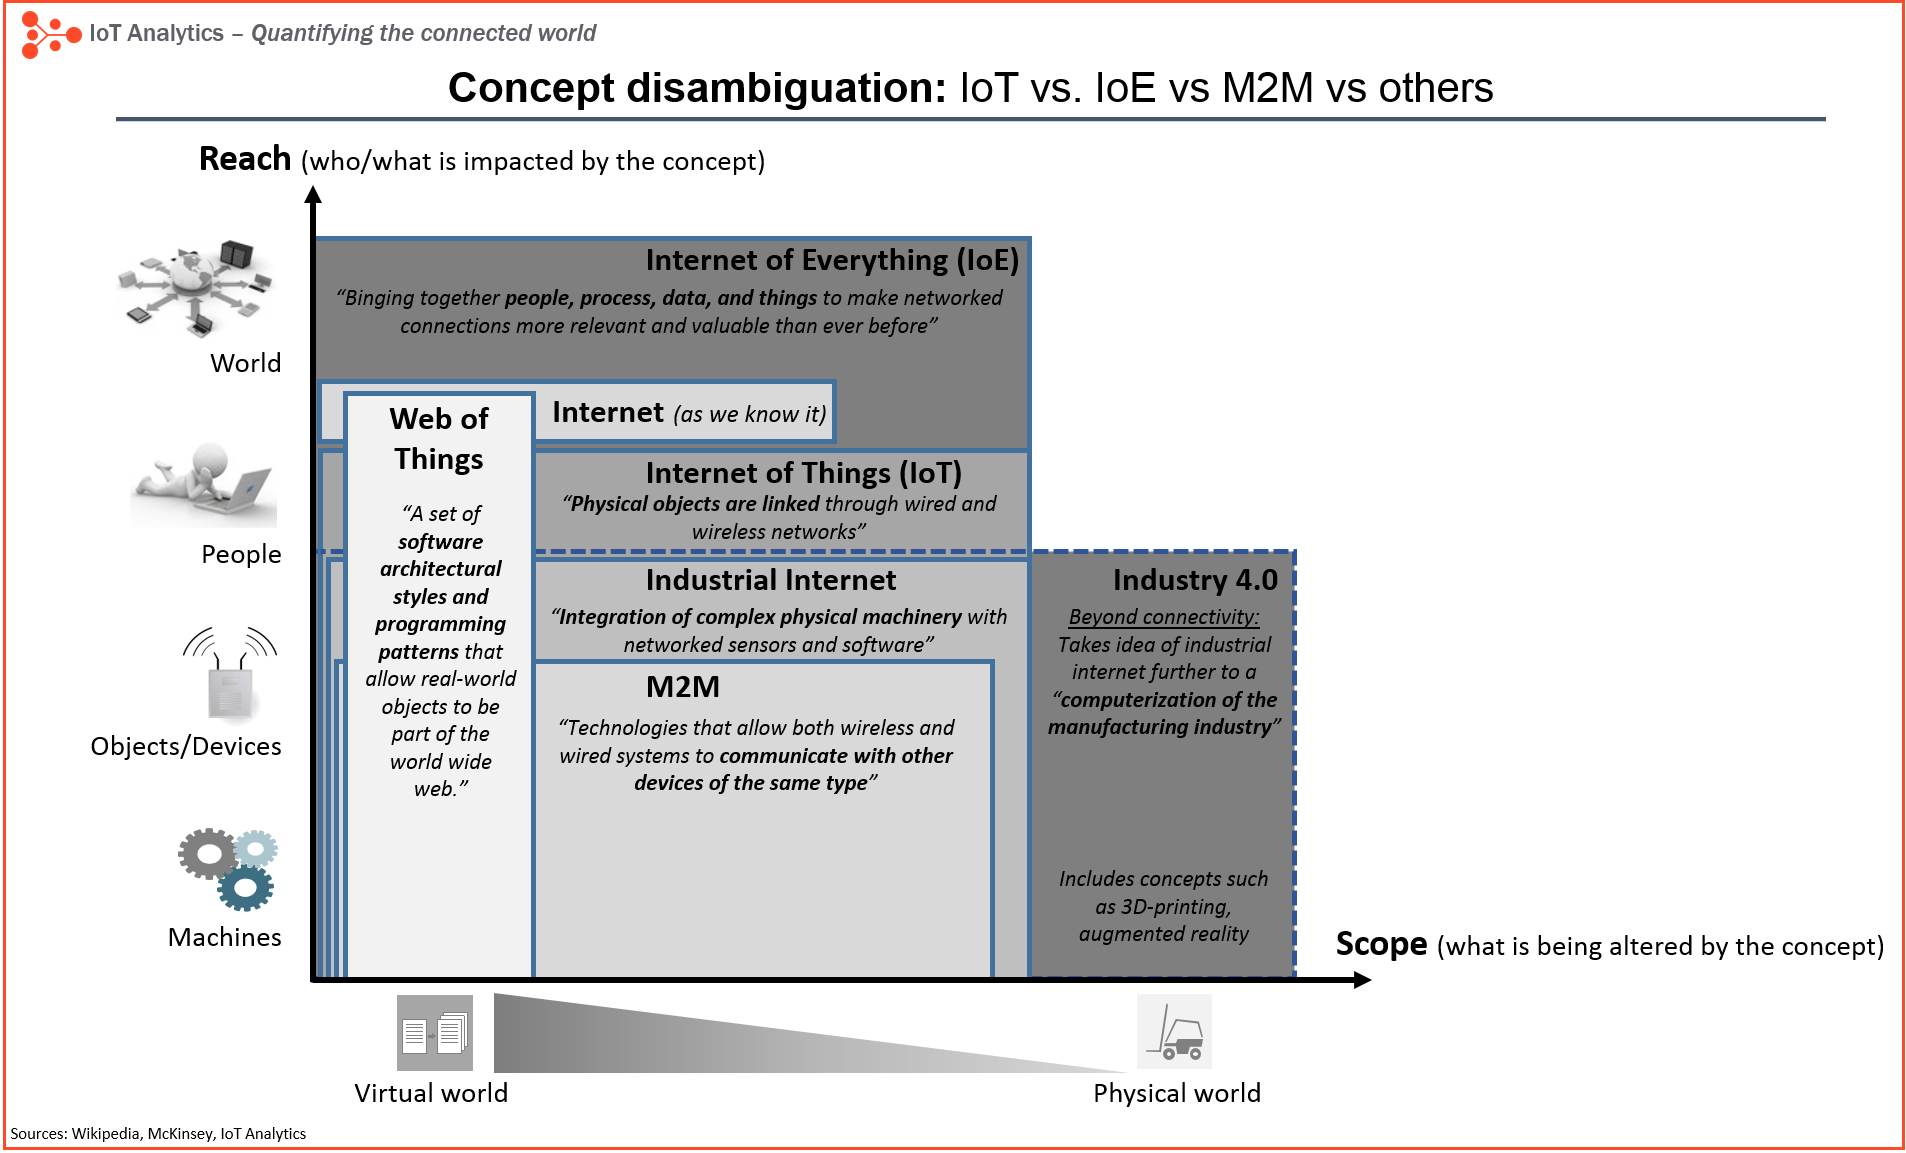
\includegraphics[scale=0.21]{imagens/outras-iot.png}}
    
    \footnotesize{Fonte:~\citet{LuethIoT2014}}
  \end{center}
\end{figure}


%%%%%%%%%%%%%%%%%%%%%%%%%%%%%%%%%%%%%%%%%%%%%%%%%%%%%%%%%%%%%%%%%%%%%%%%%%%%%%%%%
%%%%%%%%%%%%%%%%%%%%%%%%%%%%%%%%%%%%%%%%%%%%%%%%%%%%%%%%%%%%%%%%%%%%%%%%%%%%%%%%%
%%%%%%%%%%%%%%%%%%%%%%%%%%%%%%%%%%%%%%%%%%%%%%%%%%%%%%%%%%%%%%%%%%%%%%%%%%%%%%%%%
\section{Aplicações da IoT}
\label{aplicacoes-iot}

Sem dúvida nenhuma as áreas nas quais a IoT pode ser aplicada são limitadas apenas
pela imaginação humana, variando desde um simples eletrodoméstico até grandes
sistemas industriais ou sistemas para cidades inteiras.

O potencial é tão grande que ``é impossível antecipar
todas as mudanças sociais que podem ser criadas atraves da conexão de bilhões
de dispositivos''~\citep[][p.\ 18]{UKGOSWalportIoT2014}.

De modo geral os autores~\citep{OliverWymanIoT2015,UKGOSWalportIoT2014,IEEEIoTReport,IEEEIoTDefinition,ChuiIoT2010,BughinExecutiveIoT2015,GuptaMcKinseyIoT2017,McKinseyIoTHype,SAPFutureIoT,SASIoTUseCases2016} citam as seguintes grandes
áreas como as que mais se beneficiarão da aplicação da IoT --- ver também
Figuras~\ref{fig:aplicacoes-iot-1} (página~\pageref{fig:aplicacoes-iot-1}), \ref{fig:aplicacoes-iot-2}
(página~\pageref{fig:aplicacoes-iot-2}) e \ref{fig:aplicacoes-iot-3} (página~\pageref{fig:aplicacoes-iot-3}):

\begin{itemize}[noitemsep]
\item Saúde;
\item Agricultura;
\item Construção civil;
\item Varejo;
\item Energia, petróleo, gás e mineração;
\item Indústria;
\item Mobilidade e transporte (incluindo veículos autônomos);
\item Telecomunicações;
\item Serviços financeiros;
\item Escritórios;
\item Logística;
\item Entretenimento;  
\item Mídia;
\item Cidades inteligentes.
\end{itemize}

\begin{figure}[!h]
  \begin{center}
    \caption{Principais aplicações da IoT}
    \label{fig:aplicacoes-iot-1}
    \fbox{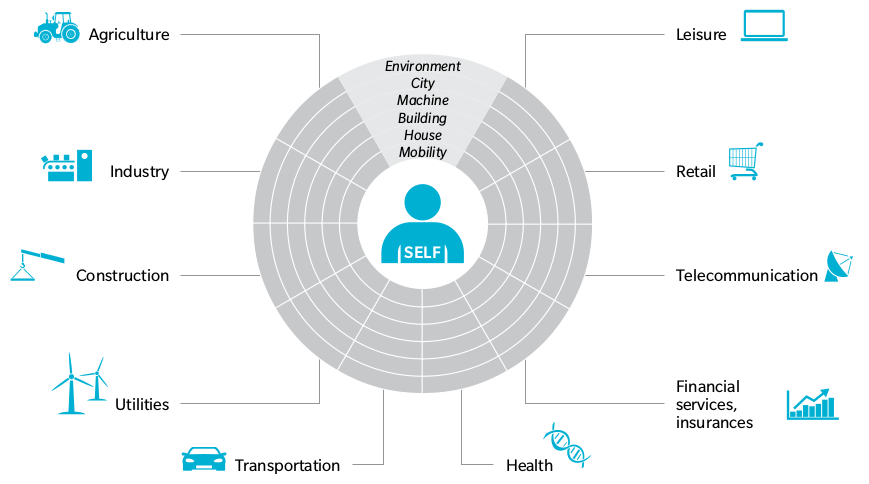
\includegraphics[scale=0.4]{imagens/aplicacoes-1.png}}
    
    \footnotesize{Fonte:~\citet[][p.\ 5]{OliverWymanIoT2015}}
  \end{center}
\end{figure}

\begin{figure}[!h]
  \begin{center}
    \caption{Principais setores beneficiados pela IoT
      e seus \ingles{stakeholders} mais importantes}
    \label{fig:aplicacoes-iot-2}
    \fbox{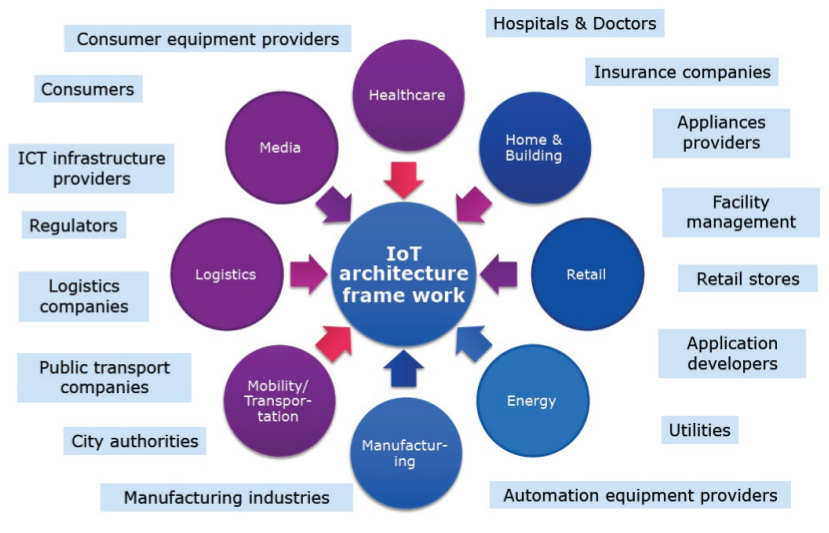
\includegraphics[scale=0.42]{imagens/aplicacoes-2.png}}
    
    \footnotesize{Fonte:~\citet[][p.\ 12]{IEEEIoTDefinition}}
  \end{center}
\end{figure}

\begin{figure}[!h]
  \begin{center}
    \caption{Principais áreas de aplicação da IoT}
    \label{fig:aplicacoes-iot-3}
    \fbox{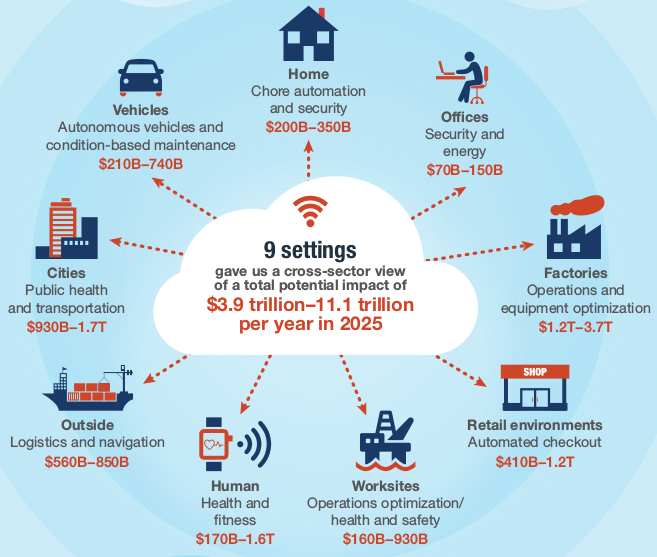
\includegraphics[scale=0.5]{imagens/aplicacoes-3.png}}
    
    \footnotesize{Fonte:~\citet[][p.\ 5]{McKinseyIoTHype}}
  \end{center}
\end{figure}

As próximas seções detalharão como a IoT causará um impacto benéfico, e mostrarão
alguns casos de sucesso que ilustram todo o potencial dessa nova tecnologia.


%%%%%%%%%%%%%%%%%%%%%%%%%%%%%%%%%%%%%%%%%%%%%%%%%%%%%%%%%%%%%%%%%%%%%%%%%%%%%%%%%
%%%%%%%%%%%%%%%%%%%%%%%%%%%%%%%%%%%%%%%%%%%%%%%%%%%%%%%%%%%%%%%%%%%%%%%%%%%%%%%%%
\subsection{Como a IoT cria valor?}
\label{aplicacoes-iot-criacao-valor}

Antes de discutirmos casos concretos da aplicação da IoT, é importante ter clara
a noção de como a IoT cria valor, ou seja, como uma rede de coisas conectadas
pode beneficiar as pessoas e gerar valor para elas e para as empresas.

Basicamente existem dois grandes ``grupos'' de atividades através das quais
as aplicações da IoT podem gerar valor~\citep{ChuiIoT2010}:
um grupo de \textbf{Informação e Análise} (que envolve atividades
de monitoramento de comportamento, obtenção de consciência em tempo real do ambiente
físico e a tomada de decisões baseadas em \emph{analytics} de sensores), e
um grupo de \textbf{Automação e Controle} (que envolve atividades de otimização
de processos, otimização do consumo de recursos e o desenvolvimento de sistemas
autônomos complexos).

Explicando melhor como a IoT gera valor, \citet{ChuiIoT2010} nos fornece
as seguintes informações e detalhes:

\begin{itemize}
\item \emph{\textbf{Informação e Análise}}: a IoT pode fornecer mais e melhor
  informação e análise, aumentando a velocidade e a performance da tomada de
  decisão. Isso é obtido através de:
  \begin{itemize}
  \item \emph{Monitoramento de comportamento}: inclui as atividades
    de monitoramento do comportamento, status e outras variáveis de pessoas,
    coisas ou dadados, no espaço e tempo. Por exemplo: uma empresa de seguros
    pode colocar sensores em carros e monitorar como e por onde um carro trafega,
    podendo basear políticas de preços personalizadas com essa informação; empresas
    podem monitorar a movimentação de produtos por toda a cadeia de suprimentos,
    melhorando o controle de estoque e reduzindo perdas;
  \item \emph{Obter consciência em tempo real do ambiente físico}: inclui as
    atividades que visam obter dados, em tempo real, de sensores alocados em
    diversas coisas ou lugares, para fornecer aos tomadores de decisão uma visão
    em tempo real do ambiente. Por exemplo: sensores sônicos espalhados pela cidade
    podem fornecer às delegacias de polícia dados instantâneos sobre a localização
    em tempo real de disparos de arma de fogo;
  \item \emph{Decisões orientadas por} analytics \emph{baseada em sensores}: a
    obtenção de dados em tempo real e sua ligação à sistema de análises automatizados
    pode orientar decisões humanas ou automáticas em diversos serviços e áreas de
    aplicação. Por exemplo: varejistas podem monitorar através de sensores a
    movimentação de clientes pela loja, verificando quais produtos os clientes
    gastam mais tempo observando, e disparar promoções ou propagandas imediatas.
  \end{itemize}
\item \emph{\textbf{Automação e Controle}}: a IoT pode criar uma base para
  automação e controle convertendo os dados obtidos pelos sensores em \emph{feedback}
  para os atuadores para a otimização e ajuste de diversos processos. Isso é obtido
  através de:
  \begin{itemize}
  \item \emph{Otimização de processos}: inclui as atividades que visam obter
    de sensores informações importantes sobre processos, analisá-las automaticamente
    e ajustar o processo para otimizá-lo em tempo real. Por exemplo: uma indústria
    pode instalar sensores de temperatura para manter sempre na faixa adequada
    um forno utilizado na produção;
  \item \emph{Otimização do consumo de recursos}: inclui as atividades que podem
    auxiliar a mudar e otimizar o uso de recursos, incluindo energia, água e
    demais recursos. Por exemplo: uma empresa de energia pode fornecer medidores
    de consumo elétrico que mostram, em tempo real, o consumo e o custo imediato
    de fornecimento, cobrando diferentemente pelo padrão e horário de uso;
  \item \emph{Sistemas autônomos complexos}: inclui as atividades que envolvem
    a rápida detecção em tempo real de condições imprevisíveis e respostas
    instantâneas guiadas por sistemas automáticos que imitam as reações humanas
    (e escolhem a melhor reação entre várias possíveis). Por exemplo: montadoras
    estão desenvolvendo vários tipos de sistemas de caros, desde sistemas de
    detecção e evasão de colisões, até carros autônomos.
  \end{itemize}
\end{itemize}

As possibilidades de geração de valor com a IoT são enormes e, à medida
em que usos mais inovadores dos sensores e dos dados forem
desenvolvidos, outros modelos de negócios e formas de geração de valor serão
criados e implementados.


%%%%%%%%%%%%%%%%%%%%%%%%%%%%%%%%%%%%%%%%%%%%%%%%%%%%%%%%%%%%%%%%%%%%%%%%%%%%%%%%%
%%%%%%%%%%%%%%%%%%%%%%%%%%%%%%%%%%%%%%%%%%%%%%%%%%%%%%%%%%%%%%%%%%%%%%%%%%%%%%%%%
\subsection{Exemplos atuais de aplicação da IoT}
\label{aplicacoes-iot-exemplos}

Devido às inúmeras aplicações da IoT já citadas na Seção~\ref{aplicacoes-iot},
apresentaremos aqui apenas alguns exemplos em três áreas: cuidados de saúde,
agricultura e transporte. Diversos outros exemplos podem ser obtidos consultando-se
as referências bibliográficas indicadas\footnote{\citet{OliverWymanIoT2015},
  \citet{UKGOSWalportIoT2014}, \citet{IEEEIoTReport}, \citet{IEEEIoTDefinition},
  \citet{ChuiIoT2010}, \citet{BughinExecutiveIoT2015}, \citet{GuptaMcKinseyIoT2017},
  \citet{McKinseyIoTHype}, \citet{SAPFutureIoT}, \citet{SASIoTUseCases2016},
  \citet{MorganStanleyIoTnow2013}, \citet{AlaskaIoTComm2015}, \citet{BackDeckerIoT2014},
  \citet{MazakIoT2016}, \citet{CopenhagenIoT2013}, \citet{KansasIoT2016},
  \citet{RockwellIoT2016}, \citet{MississaugaIoT2015}}.


%%%%%%%%%%%%%%%%%%%%%%%%%%%%%%%%%%%%%%%%%%%%%%%%%%%%%%%%%%%%%%%%%%%%%%%%%%%%%%%%%
\subsubsection{Cuidados de saúde}
\label{aplicacoes-iot-exemplos-saude}

A IoT nos cuidados de saúde ``pode ajudar
a mudar o foco da cura para a prevenção e dar às pessoas maior controle sobre
as decisões que afetam seu bem-estar''~\citep[][p.\ 29]{UKGOSWalportIoT2014}.
Algumas aplicações já existem:

\paragraph{Ambulâncias aéreas} A \ingles{California Shock Trauma Air Rescure (CALSTAR)}
é um serviço de ambulância aérea que começou a utilizar conceitos de IoT para
integrar sistemas de comunicação ar-solo para conectar suas aeronavas de
transporte às instituições de saúde~\citep{CiscoCALSTAR}.

\paragraph{Aplicativos \emph{fitness}} Diversos aplicativos voltados para saúde
e \emph{fitness} já existem, alguns conectados à sensores IoT que captam
dados como freqüência cardíaca. Os dez maiores aplicativos desse gênero
estão realmente contribuindo para tornar mais saudáveis os hábitos
de saúde de seus usuários~\citep{OliverWymanIoT2015}.

\paragraph{Monitoramento contínuo} Usando soluções de monitoramento contínuo,
a IoT está aumentando a aderência dos pacientes às terapias prescritas, diminuindo
as internações e aumentanto a qualidade de vida de pacientes~\citep{McKinseyIoTHype}.


%%%%%%%%%%%%%%%%%%%%%%%%%%%%%%%%%%%%%%%%%%%%%%%%%%%%%%%%%%%%%%%%%%%%%%%%%%%%%%%%%
\subsubsection{Agricultura}
\label{aplicacoes-iot-exemplos-agricultura}

Aplicações da IoT na área de agricultura são diversas e com potencial de aumentar
a produtividade alimentar e aumentar a proteção ao meio ambiente. Algumas
iniciativas interessantes:

\paragraph{Monitoramento de colméias} Soluções de IoT já são utilizadas para
monitorar colméias de abelhas em tempo real, reduzindo a inspeção manual que causa
distúrbios nas colméias e diminuem a produtividade de mel~\citep{SilvaIoTColmeia2017}.

\paragraph{Sistemas de irrigação} Já existem sistemas de irrigação baseados em IoT
que, através de sensores de umidade do solo, temperatura e umidade do ar, conseguem
otimizar e setorializar a irrigação de lavouras~\citep{UKGOSWalportIoT2014}. Aplicações
domésticas para irrigação de jardins também existem~\citep{GrehsIrrigacaoIoT2016}.

\paragraph{Monitoramento de gado} Soluções para monitoramento em tempo real de gado,
através de dispositivos ligados ao Sistema de Posicionamento Global (\emph{Global
  Positioning System} --- GPS) permitem entender o comportamento de rebanhos e
identificar animais machucados ou doentes~\citep{SpinkIoTTrackAnimals2013}.


%%%%%%%%%%%%%%%%%%%%%%%%%%%%%%%%%%%%%%%%%%%%%%%%%%%%%%%%%%%%%%%%%%%%%%%%%%%%%%%%%
\subsubsection{Transporte e mobilidade}
\label{aplicacoes-iot-exemplos-transporte}

Diversas iniciativas interessantes existem na área de transporte e mobilidade,
e o potencial para veículos autônomos é enorme. Algumas iniciativas interessantes:

\paragraph{Avisos de alteração nos sinais de trânsito} A cidade de \ingles{Newcastle}
está testando um sistema baseado em IoT que sinaliza aos motoristas que é o momento
de ajustar a velocidade do carro (aumentar ou diminuir) se as luzes dos sinais
de trânsito estão prestes a mudar~\citep{UKGOSWalportIoT2014}.

\paragraph{Transporte escolar inteligente} A \ingles{Watkins Glen Central School District},
em \ingles{New York}, implantou um projeto de IoT para conectar os ônibus escolares
à escola, tornando-os uma espécie de campus escolar digital. Isso foi feito pois muitos
alunos realizam viagens de quase uma hora nesses ônibus e, para estimular a realização
das tarefas de casa, os professores passaram a implementar atividades para serem feitas
nos ônibus, no trajeto entre a escola e a residência dos alunos~\citep{GlenSchoolBusIoT2016}.

\paragraph{Estradas que previnem engarrafamentos} Na Áustria, recentemente,
a empresa pública \ingles{Autobahnen- und Schnellstraßen-Finanzierungs-Aktiengesellschaft} (ASFiNAG) --- que
é a resposável pela manutenção das autoestradas --- implantou uma
rede de mais de 70 mil sensores de movimento e localização em todas as autoestradas
austríacas. Essa rede de sensores é capaz de identificar e prevenir
a formação de engarrafamentos, além de identificar veículos com
problemas~\citep{ASFiNAGIoT2015}.


%%%%%%%%%%%%%%%%%%%%%%%%%%%%%%%%%%%%%%%%%%%%%%%%%%%%%%%%%%%%%%%%%%%%%%%%%%%%%%%%%
\subsubsection{Aplicações ``triviais''}
\label{aplicacoes-iot-exemplos-triviais}

Além dos exemplos fornecidos nas seções anteriores, que procuram demonstrar a
vanguarda da inovação em IoT, diversas aplicações mais triviais (mas não menos
importantes) também existem. Alguns exemplos que já fazem parte de nosso cotidiano
incluem, por exemplo: a) sistemas de sensoriamento e localização de vagas em
estacionamentos; b) sistemas de \ingles{Smart-TVs} interativas; c) relógios
inteligentes; d) irrigação de plantações; e e) controle ambiente de temperatura.



%%%%%%%%%%%%%%%%%%%%%%%%%%%%%%%%%%%%%%%%%%%%%%%%%%%%%%%%%%%%%%%%%%%%%%%%%%%%%%%%%
%%%%%%%%%%%%%%%%%%%%%%%%%%%%%%%%%%%%%%%%%%%%%%%%%%%%%%%%%%%%%%%%%%%%%%%%%%%%%%%%%
%%%%%%%%%%%%%%%%%%%%%%%%%%%%%%%%%%%%%%%%%%%%%%%%%%%%%%%%%%%%%%%%%%%%%%%%%%%%%%%%%
\section{Riscos e perigos da IoT}
\label{perigos-iot}


%%%%%%%%%%%%%%%%%%%%%%%%%%%%%%%%%%%%%%%%%%%%%%%%%%%%%%%%%%%%%%%%%%%%%%%%%%%%%%%%%
%%%%%%%%%%%%%%%%%%%%%%%%%%%%%%%%%%%%%%%%%%%%%%%%%%%%%%%%%%%%%%%%%%%%%%%%%%%%%%%%%
\subsection{Problemas de segurança e privacidade}
\label{perigos-iot-seguranca-privacidade}

Sem dúvida nenhuma os principais questionamentos quanto aos perigos e riscos
da IoT referem-se a \textbf{segurança} dos dispositivos e \textbf{privacidade} dos
dados e/ou pessoas~\citep{BauerMcKinseyIotSecurity2017,HuSecurityIoT2016,SANSMilleyIoT2017,SansPescatoreIoT2014,SANSRivasIoT2017,RussellIoTSecurity2016}.

Conectar bilhões de dispositivos à Internet significa dizer que \ingles{hackers}
terão à sua disposição todo esse parque tecnológico como possível alvo de
ataque cibernético. Esses ataques podem variar de \emph{simples inconvenientes} (um
ataque a uma \ingles{Smart-TV} ou a um regulador de temperatura de um ar-condicionado),
até \emph{situações onde a própria vida das pessoas é ameaçada} (um ataque a aparelhos
de marca-passos cardíacos). Esta última situação é tão preocupante que levou a
\ingles{Food and Drug Administration} (FDA) a exigir um \ingles{recall} de 500 mil
marca-passos cardíacos, de diversos fabricantes, que já estavam em uso em pacientes
americanos, devido à constatação de que os mecanismos de conectividade à Internet
nesses aparelhos apresentavam baixa segurança e poderiam ser alvo de ataques
\ingles{hackers} que poderiam até causar a morte por alteração da
freqüência cardíaca~\citep{HernPacemakersIoTRecall2017}.

Ainda não existe um padrão de segurança para dispositivos IoT que seja considerado
totalmente adequado: cada fabricante tenta estabelecer mecanismos de segurança
próprios. O problema é que esses mecanismos de segurança muitas vezes não são
tão seguros assim e deixar que cada fabricante estabeleça seu mecanismo de proteção
pode, a longo prazo, influenciar na capacidade de interligação dos dispositivos IoT
prejudicando o próprio conceito e utilidade de manter coisas conectadas.

Enquanto não for estabelecido um ``padrão ouro'' para a segurança de dispositivos
IoT, pelo menos para os mais críticos (como os marca-passos cardíacos, por
exemplo), a adoção da tecnologia trará muitos riscos e sofrerá de imensa
desconfiança pelo público.

Outro problema relacionado à segurança diz respeito à privacidade de dados e
das pessoas. As pessoas ainda não têm total consciência do fato mas todo mundo
está sendo monitorado e rastreado o tempo todo: os telefones celulares tranmitem
dados de localização em tempo real; os cartões de crédito transmitem todas as
suas compras; supermercados transmitem seus dados de compra para o governo;
sua \ingles{Smart-TV} ou um serviço como o \ingles{Netflix} conhece suas
preferências e gostos de filmes; dispositivos IoT para segurança doméstica
transmitem o horário que uma pessoa chega ou sai de casa; sensores de
movimento para segurança doméstica transmitem informações sobre a presença ou
não de pessoas em casa; serviços de transporte (como \ingles{Uber}) sabem quais
as rotas, origens e destinos do cotidiano das pessoas;
relógios inteligentes transmitem dados de localização;
enfim\ldots os exemplos são inúmeros.

E se hoje, com o número relativamente pequeno de dispositivos IoT, já temos
essa enorme quantidade de informações sobre as pessoas sendo transmitidas,
qual volume de dados sobre os cidadãos estará disponível em alguns anos?
Será gigantesco. E qual o problema disso? A perda total da privacidade das pessoas.

Hoje já é possível identificar uma pessoa a partir de dados teoricamente anônimos,
apenas analisando-se coisas como o padrão de navegação de sites na Internet.
Imagine uma família composta por um pai, mãe e uma criança, onde todos utilizam
um mesmo computador de forma ``anônima''. Cada membro pode ser facilmente identificado
pelo padrão de navegação em sites diferentes (o pai pode acessar mais páginas
de jornal ou futebol, a mãe de moda e educação infantil,
e a criança acessa páginas de desenhos animados).

Quando, no futuro, bilhões de dispositivos estiverem conectados e transmitindo
dados sobre as pessoas em tempo real, ferramentas de \ingles{Data Science} e
\ingles{Big Data Analytics} de tempo real poderão identificar inequivocadamente
qualquer pessoa através da identificação de \textbf{padrões de comportamente e consumo}.
Esse é o fim da privacidade como hoje a entendemos.

As pessoas estarão conscientes e prontas para isso? Você gostaria que uma
empresa ou o governo soubesse tudo o que você faz, tudo o que você compra,
todos os caminhos por onde você anda todos os dias, todas as suas consultas
e histórico médico?

A IoT pode ser potencialmente benéfica mas a facilidade com a qual, no futuro,
pode-se criar não apenas um único ``\ingles{Big Brother}'', mas vários,
nos assusta e nos lembra imediatamente de George Orwell e sua distopia
totalitária descrita no livro \emph{1984}~\citep{Orwell1984}.


%%%%%%%%%%%%%%%%%%%%%%%%%%%%%%%%%%%%%%%%%%%%%%%%%%%%%%%%%%%%%%%%%%%%%%%%%%%%%%%%%
%%%%%%%%%%%%%%%%%%%%%%%%%%%%%%%%%%%%%%%%%%%%%%%%%%%%%%%%%%%%%%%%%%%%%%%%%%%%%%%%%
\subsection{Problemas relacionados ao modelo de negócio}
\label{perigos-iot-modelo-negocio}

Uma outra questão que pode colocar em risco o futura da IoT não está relacionada
à segurança nem à privacidade mas, sim, ao modelo de negócio e a interferência governamental.

Hoje não se tem muito claro como, a partir do potencial da IoT, criar modelos
de negócio sustentáveis~\citep{IEEEIoTReport,UKGOSWalportIoT2014}.

Também não está claro se, e como, os governos tentarão regular e/ou burocratizar
a tecnologia, e isso é um fator de incerteza e risco, por exemplo: se os governos
determinarem que os dispositivos IoT paguem impostos em demasia ou pela
transmissão de dados, todo o ``negócio IoT'' estará em risco.

Questões legais e jurídicas, como a questão da propriedade e do uso justo
dos dados obtidos, serão cruciais no futuro.

Todas essas questões estão sendo debatidas, mas ainda não existe uma resposta
definitiva. Essa incerteza precisará ser mitigada para que a IoT possa alcançar
todo seu potencial.


%%%%%%%%%%%%%%%%%%%%%%%%%%%%%%%%%%%%%%%%%%%%%%%%%%%%%%%%%%%%%%%%%%%%%%%%%%%%%%%%%
%%%%%%%%%%%%%%%%%%%%%%%%%%%%%%%%%%%%%%%%%%%%%%%%%%%%%%%%%%%%%%%%%%%%%%%%%%%%%%%%%
%%%%%%%%%%%%%%%%%%%%%%%%%%%%%%%%%%%%%%%%%%%%%%%%%%%%%%%%%%%%%%%%%%%%%%%%%%%%%%%%%
\section{Tecnlogias para a IoT}
\label{tecnologia-iot}

Quando falamos sobre tecnologias para IoT é necessário diferenciar a tecnologia
para os dispositivos IoT, e a tecnologia para a comunicação entre os dispositivos:
esta ainda representa um risco ao ``negótio IoT'', e aquela já está bem consolidada.


%%%%%%%%%%%%%%%%%%%%%%%%%%%%%%%%%%%%%%%%%%%%%%%%%%%%%%%%%%%%%%%%%%%%%%%%%%%%%%%%%
%%%%%%%%%%%%%%%%%%%%%%%%%%%%%%%%%%%%%%%%%%%%%%%%%%%%%%%%%%%%%%%%%%%%%%%%%%%%%%%%%
\subsection{Tecnologia para os dispositivos}
\label{tecnologia-iot-dispositivos}

Os dispositivos IoT utilizam diversas tecnologias de \ingles{hardware}, incluindo
placas de circuito, microcontroladores, placas de comunicação e, principalmente,
uma gama diversa de sensores e atuadores que permitem que cada dispositivo IoT
seja manufaturado especificamente para uma determinada função, e a baixo custo.

Praticamente qualquer utilização imaginável para um dispositivo IoT já conta com
algum \ingles{hardware} específico pronto para uso, bastando-se construir a
solução desejada.

Já existem até mesmo plataformas de \ingles{hardware open-source}, como o
Arduino~\citep{McRobertsArduino2011,JavedArduinoIoT2016,SeneviratneIoTArduino2015,SchwartzESP8266IoT2016,BlumArduino2013,BoxallArduino2013,FitzgeraldShiloh2013}, ver Figura~\ref{fig:arduino-1}, que permitem a rápida prototipação e desenvolvimento de soluções
de IoT que, posteriormente, são transformadas em produtos.

\begin{figure}[!h]
  \begin{center}
    \caption{Arduino Uno Rev.\ 3}
    \label{fig:arduino-1}
    \fbox{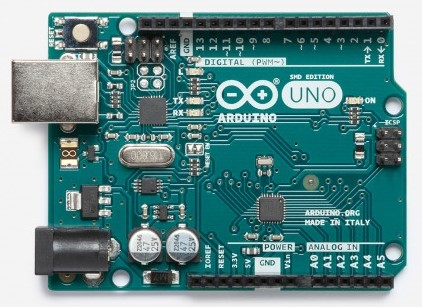
\includegraphics[scale=1.0]{imagens/arduino.jpg}}
    
    \footnotesize{Fonte:~\citet{FitzgeraldShiloh2013}}
  \end{center}
\end{figure}


%%%%%%%%%%%%%%%%%%%%%%%%%%%%%%%%%%%%%%%%%%%%%%%%%%%%%%%%%%%%%%%%%%%%%%%%%%%%%%%%%
\subsection{Tecnologia para a comunicação}
\label{tecnologia-iot-comunicacao}

Ao contrário da tecnologia para a criação dos dispositivos IoT, que já está
bem estabelecida, a tecnologia para a comunicação entre os dispositivos e
entre os dispositivos e a Internet ainda não está bem estabelecida e em um padrão
claro universal para a transmissão ainda não existe~\citep{NunesLoRaSigfox2017,AlsenMcKinseyIoT2017,LuetMcKinseyIoTPlatforms2017}.

O problema é que um sistema completo de IoT apresenta várias ``camadas''
(ver Figura~\ref{fig:camadas-iot}) sendo que duas camadas são envolvidas na comunicação de dados
e a falta de uma padronização para essa tecnologia de transmissão afeta o
impacto da IoT: de que adianta bilhões de dispositivos conectados se eles não
conseguem conversar entre si?

\begin{figure}[!h]
  \begin{center}
    \caption{Camadas de um sistema IoT}
    \label{fig:camadas-iot}
    \fbox{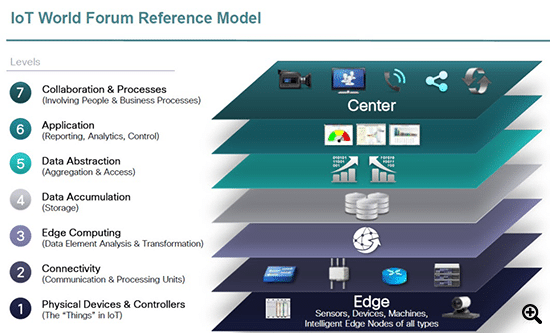
\includegraphics[scale=0.7]{imagens/camadas-iot.png}}
    
    \footnotesize{Fonte:~\citet{NunesLoRaSigfox2017}}
  \end{center}
\end{figure}

Especificamente na camada de conectividade (representado pelo ``nível 2'' na
Figura~\ref{fig:camadas-iot}) existem diversas alternativas possíveis,
algumas mais abertas do que outras, com diferentes níveis de cobertura global.
E é essa varidade de alternativas, sem um claro padrão entre elas,
que pode causar problemas futuros de intercomunicação aos dispositivos IoT.

As principais tecnologias de comunicação criadas especificamente
para redes IoT são~\citep{NunesLoRaSigfox2017,AlsenMcKinseyIoT2017}:

\begin{itemize}
\item \textbf{Rede LoRaWAN (\ingles{Low Power, Wide Area Network})}\footnote{\url{https://lora-alliance.org}}:
  é uma rede de comunicação \ingles{wireless} para conexão de dispositivos de
  baixo consumo a longas distâncias (até 15 Km). É uma arquitetura mais aberta,
  na qual cada empresa pode pagar para criar sua própria rede IoT ou usar redes de terceiros;
\item \textbf{Rede NB-IoT (\ingles{Narrow Band IoT})}\footnote{\url{https://www.gsma.com/iot/narrow-band-internet-of-things-nb-iot}}:
  é uma rede de comunicação que usará frequências 3G, 4G e 5G para a transmissão de dados;
\item \textbf{Rede \ingles{SigFox}}\footnote{\url{https://www.sigfox.com}}: 
  é uma rede de comunicação desenvolvida pela empresa \ingles{Sigfox} cujo objetivo é
  estabelecer uma cobertura global para aplicações de IoT.
\end{itemize}

Também existem soluções de IoT que utilizam padrões de rede de comunicação já estabelecidos,
como redes TCP/IP, mas que apresentam maior custo.

De qualquer forma, a falta de uma maior padronização na tecnologia de
comunicação dos dispositivos IoT é identificada por alguns autores
como um risco potencial ao ``negócio IoT''~\citep{UKGOSWalportIoT2014}.


%%%%%%%%%%%%%%%%%%%%%%%%%%%%%%%%%%%%%%%%%%%%%%%%%%%%%%%%%%%%%%%%%%%%%%%%%%%%%%%%%
%%%%%%%%%%%%%%%%%%%%%%%%%%%%%%%%%%%%%%%%%%%%%%%%%%%%%%%%%%%%%%%%%%%%%%%%%%%%%%%%%
%%%%%%%%%%%%%%%%%%%%%%%%%%%%%%%%%%%%%%%%%%%%%%%%%%%%%%%%%%%%%%%%%%%%%%%%%%%%%%%%%
\section{Prova de conceito: Cofre-IoT}
\label{cofre-iot}

Como prova de conceito de um dispositivo IoT os autores deste Trabalho Acadêmico
desenvolverão um cofre conectado --- Cofre-IoT --- que será capaz de armazenar
valores e fornecer como serviço um \ingles{website} ou aplicativo \ingles{mobile}
para que o usuário possa acompanhar sua meta de economia financeira.

As funcionalidades planejadas para o Cofre-IoT são:

\begin{itemize}
\item \textbf{Fechadura}: não utilizará chaves ou trancas mecânicas para
  combinação de segredo. A porta do cofre será aberta mediante a identificação
  biométrica da impressão digital do usuário (as impressões digitais
  dos dedos do usuário ficarão armazenadas localmente);
\item \textbf{\ingles{Display}}: existirá um \ingles{display} capaz de mostrar
  a quantidade de dinheiro em seu interior. Esse \ingles{display} somente será
  acionado enquanto a porta estiver aberta, após a identificação biométrica do usuário;
\item \textbf{Teclado numérico}: o cofre terá um teclado numérico simples,
  capaz de realizar operações de adição e subtração, para que o usuário informe
  a quantidade de dinheiro acrescentado ou retirado do cofre;
\item \textbf{Conexão \ingles{wireless}}: existirá algum mecanismo de conexão
  \ingles{wireless} para que o Cofre-IoT possa enviar os dados de depósito ou
  saque para o serviço em nuvem que controlará a meta financeira do usuário.
  Essa conexão \ingles{wireless} também enviará registros de abertura do cofre
  para um \ingles{log} de acesso;
\item \textbf{Site de finanças pessoal}: o cofre armazenará as informações
  financeiras e oferecerá um serviço de poupança e finanças pessoais em nuvem
  (no endereço https://www.cofreiot.com.br)\footnote{%
    Outras opções de domínio também serão avaliadas como, por exemplo:
    \begin{itemize}[noitemsep]
    \item https://www.cofre-iot.com.br
    \item https://www.cofrenanet.com.br
    \item https://www.minhapoupancapessoal.com.br
    \item https://www.poupancapessoal.com.br
    \item https://www.poupancaiot.com.br
    \end{itemize}}
  para que o próprio usuário estabeleça suas metas de poupança e em quanto
  tempo ele gostaria de alcançar a economia pretendida. O sistema sugerirá
  um cronograma de depósitos adequado;
\item \textbf{Aplicativo \ingles{mobile}}: poderá ser desenvolvido um
  aplicativo \ingles{mobile} que informe o progresso financeiro do
  usuário e alerte a abertura do cofre.
\end{itemize}

Utilizaremos como tecnologia de prototipagem do cofre o Arduino com alguma
placa \ingles{shield} de conexão \ingles{wireless}.

O \ingles{backend} do sistema estará localizado em um provedor de serviços em nuvem
(\ingles{Amazon AWS}) e será desenvolvido sobre um sistema \ingles{Linux} (\ingles{CentOS})\footnote{\url{https://www.centos.org/}},
com um banco de dados de alta performance (\ingles{Oracle})\footnote{\url{https://www.oracle.com/database/}},
e um servidor \ingles{web} para proporcionar a conexão com o cofre (\ingles{Apache})\footnote{\url{https://httpd.apache.org/}}.

O \ingles{frontend desktop} será fornecido por uma aplicação responsiva (os autores
consideram utilizar um sistema de desenvolvimento rápido (\ingles{Oracle Apex})\footnote{\url{https://apex.oracle.com/}}
nessa fase da prototipagem) que permite ao usuário acompanhar sua meta financeira
e conhecer o melhor cronograma de depósitos para alcançar essa meta.
Obviamente o cofre também informará ao usuário as perdas que ele terá devido
à inflação ao optar por guardar dinheiro em casa, num cofre.

Outro \ingles{frontend} para aplicativos \ingles{mobile} etá planejado, mas talvez
só seja possível desenvolver essa funcionalidade em versões futuas do cofre
(a idéia aqui é apenas criar uma prova de conceito da IoT, não um sitema
totalmente funcional e pronto para comercialização).

Não serão levadas em conta questões relativas ao custo/benefício do desenvolvimento
do Cofre-IoT pois, novamente, esse ``produto'' é apenas uma prova de conceito.

Todos os materiais de referência, esquemas, padrões, códigos, programas e textos
referentes ao desenvolvimento do Cofre-IoT (inclusive o texto original deste Trabalho
Acadêmico em formatos para o \ingles{Microsoft Word}\footnote{O formato para o Microsoft Word
  (\url{https://products.office.com/pt-br/word}) tem a única função de manter a apresentação
  gráfica deste Trabalho Acadêmico dentro das regras de normalização de trabalho
  da FAESA Centro Universitário. Não será atualizado.} e para o \LaTeX\footnote{O formato para o \LaTeX
  (\url{https://www.latex-project.org}) é o formato padrão para o \ingles{typesetting} de publicações
  deste projeto, e para a produção, comunicação e divulgação de toda a documentação
  técnica e/ou científica produzida referente ao Cofre-IoT. Será atualizado.}) já estão disponíveis
para acesso e consulta pública no repositório \ingles{GitHub} do projeto em:
\url{https://github.com/abrantesasf/cofre-IoT/}.

A Figura~\ref{fig:arquitetura-cofre-iot} exibe o primeiro rascunho resultante de \ingles{brainstorming}
realizado pelos autores para a definição de uma primeira proposta de arquitetura IoT
para o cofre. Alterações na arquitetura proposta serão informadas e divulgadas
no repositório \ingles{GitHub} do projeto\footnote{\url{https://github.com/abrantesasf/cofre-IoT/}}.

\begin{figure}[!h]
  \begin{center}
    \caption{Primeiro rascunho de arquitetura IoT para o cofre}
    \label{fig:arquitetura-cofre-iot}
    \fbox{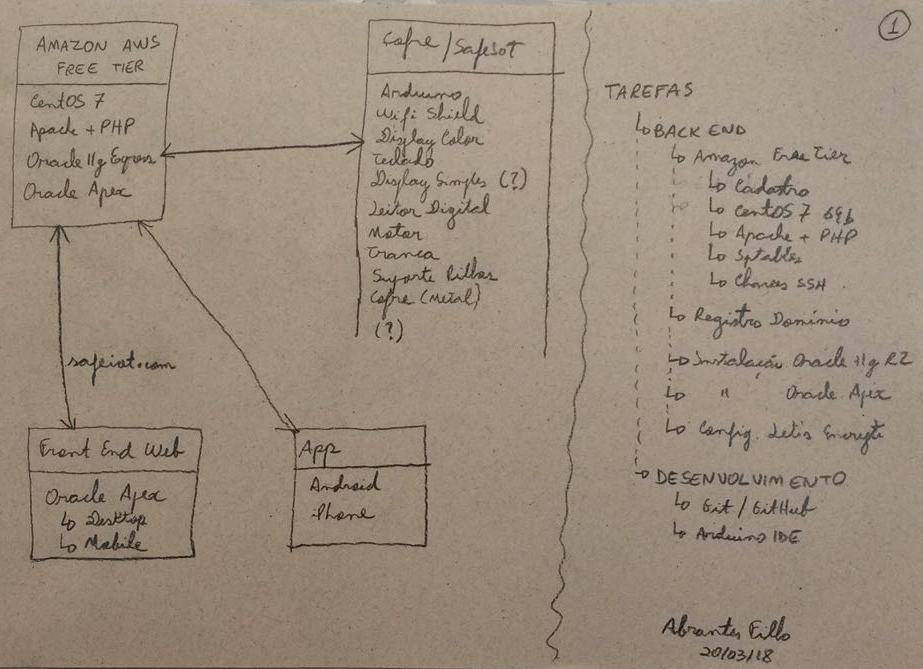
\includegraphics[scale=0.42]{imagens/arquitetura-01.jpg}}
    
    \footnotesize{Fonte: produzido pelos autores}
  \end{center}
\end{figure}


%%%%%%%%%%%%%%%%%%%%%%%%%%%%%%%%%%%%%%%%%%%%%%%%%%%%%%%%%%%%%%%%%%%%%%%%%%%%%%%%%
%%%%%%%%%%%%%%%%%%%%%%%%%%%%%%%%%%%%%%%%%%%%%%%%%%%%%%%%%%%%%%%%%%%%%%%%%%%%%%%%%
%%%%%%%%%%%%%%%%%%%%%%%%%%%%%%%%%%%%%%%%%%%%%%%%%%%%%%%%%%%%%%%%%%%%%%%%%%%%%%%%%
\section{Conclusão}
\label{conclusao}

A Internet das Coisas é um novo paradigma no uso da tecnologia de dispositivos
conectados à rede que proporciona o desenvolvimento de aplicações, serviços e
interatividade em diversas áreas. O potencial para a geração de valor direto para
as pessoas e para empresas é imenso.

Entretanto, ainda não se tem muito claro todo o impacto que a IoT pode proporcionar
pois é uma tecnologia relativamente recente e, apesar das inúmeras aplicações potenciais,
ainda é cedo para avaliar se a relação custo/benefício proporcionará a evolução de
modelos de negócio sustentáveis (principalmente nos ecossistemas de grande escala).
Criar inovação em uma área como a IoT é relativamente fácil: praticamente já existe tecnologia
para transformar qualquer idéia em um produto; o difícil é saber se esse produto
resultará em um negócio sustentável no futuro.

Além disso, questões de segurança e privacidade das informações também precisam
ser melhoradas antes que a IoT possa ser adotada em escala global, com a
conexão de milhões ou bilhões de dispositivos em uma única ``grande rede de IoT''.

Quando os perigos e riscos inerentes ao uso dessa nova tecnologia forem minimizados,
a IoT poderá alcançar todo seu potencial em um ecossistema de grande escala.
Até lá os principais sistemas IoT serão de pequena escala e os criados por um único
fabricante para aplicações específicas e localizadas.


%%%%%%%%%%%%%%%%%%%%%%%%%%%%%%%%%%%%%%%%%%%%%%%%%%%%%%%%%%%%%%%%%%%%%%%%%%%%%%%%%
%%%%%%%%%%%%%%%%%%%%%%%%%%%%%%%%%%%%%%%%%%%%%%%%%%%%%%%%%%%%%%%%%%%%%%%%%%%%%%%%%
%%%%%%%%%%%%%%%%%%%%%%%%%%%%%%%%%%%%%%%%%%%%%%%%%%%%%%%%%%%%%%%%%%%%%%%%%%%%%%%%%
%%%%%%%%%%%%%%%%%%%%%%%%%%%%%%%%%%%%%%%%%%%%%%%%%%%%%%%%%%%%%%%%%%%%%%%%%%%%%%%%%
%%%%%%%%%%%%%%%%%%%%%%%%%%%%%% TERMINA O DOCUMENTO %%%%%%%%%%%%%%%%%%%%%%%%%%%%%%
%%%%%%%%%%%%%%%%%%%%%%%%%%%%%%%%%%%%%%%%%%%%%%%%%%%%%%%%%%%%%%%%%%%%%%%%%%%%%%%%%
%%%%%%%%%%%%%%%%%%%%%%%%%%%%%%%%%%%%%%%%%%%%%%%%%%%%%%%%%%%%%%%%%%%%%%%%%%%%%%%%%
%%%%%%%%%%%%%%%%%%%%%%%%%%%%%%%%%%%%%%%%%%%%%%%%%%%%%%%%%%%%%%%%%%%%%%%%%%%%%%%%%
%%%%%%%%%%%%%%%%%%%%%%%%%%%%%%%%%%%%%%%%%%%%%%%%%%%%%%%%%%%%%%%%%%%%%%%%%%%%%%%%%
\bibliography{/home/abrantesasf/repositoriosGit/BibTeX/biblioteca}
\end{document}
